\documentclass[11pt,a4paper]{article}
\usepackage{fontspec}
\usepackage{unicode-math}
\setmainfont{texgyrepagella-regular.otf}[BoldFont=texgyrepagella-bold.otf,ItalicFont=texgyrepagella-italic.otf,BoldItalicFont=texgyrepagella-bolditalic.otf]
\setmathfont{texgyrepagella-math.otf}
\usepackage{amsmath}
\usepackage[a4paper,margin=2.5cm]{geometry}
\usepackage{microtype,booktabs,tabularx,array,enumitem,titlesec}
\usepackage{tikz}
\usetikzlibrary{arrows.meta,positioning}
\usepackage[unicode,hidelinks]{hyperref}
\hypersetup{pdftitle={Sổ tay đọc đề và tư duy giải Vật lý điện tử - Chương 1, 2, 3},pdfauthor={Tài liệu trợ giảng PH3330},pdfsubject={Khái niệm, ký hiệu, mô hình và đường đi từ dữ kiện tới đáp số}}
\linespread{1.06}
\setlength{\parindent}{0pt}
\setlength{\parskip}{5pt plus 1pt minus 1pt}
\setlength{\emergencystretch}{2em}
\setlength{\abovedisplayskip}{6pt plus 2pt minus 1pt}
\setlength{\belowdisplayskip}{6pt plus 2pt minus 1pt}
\setlist{leftmargin=1.5em,itemsep=2pt,topsep=3pt,parsep=0pt}
\titleformat{\section}{\Large\bfseries}{\thesection.}{0.5em}{}
\titleformat{\subsection}{\large\bfseries}{\thesubsection.}{0.5em}{}
\titleformat{\subsubsection}{\normalsize\bfseries}{}{0pt}{}
\titlespacing*{\section}{0pt}{12pt}{8pt}
\titlespacing*{\subsection}{0pt}{11pt}{5pt}
\titlespacing*{\subsubsection}{0pt}{7pt}{3pt}
\renewcommand{\arraystretch}{1.22}
\renewcommand{\contentsname}{Mục lục}
\setcounter{tocdepth}{2}
\setlength{\tabcolsep}{5pt}
\newcolumntype{Y}{>{\raggedright\arraybackslash}X}
\newcolumntype{Q}[1]{>{\raggedright\arraybackslash}p{#1}}
\newcommand{\unit}[1]{\,\mathrm{#1}}
\newcommand{\key}[1]{\textbf{#1}}
\newcommand{\idea}[1]{\par\textbf{Hiểu bằng lời.} #1\par}
\newcommand{\readit}[1]{\par\textbf{Đọc đề.} #1\par}
\newcommand{\think}[1]{\par\textbf{Tư duy ngược.} #1\par}
\newcommand{\trap}[1]{\par\textbf{Chỗ dễ nhầm.} #1\par}
\newcommand{\checkit}[1]{\par\textbf{Tự kiểm tra.} #1\par}
\newcommand{\ex}[1]{\subsubsection*{Ví dụ đọc đề: #1}}
\newcommand{\chap}[1]{\par\section{#1}}
\pagestyle{plain}
\begin{document}
\begin{center}
{\LARGE\bfseries SỔ TAY ĐỌC ĐỀ VÀ TƯ DUY GIẢI}\\[5pt]
{\Large Vật lý điện tử - Chương 1, 2, 3}\\[6pt]
{\normalsize PH3330 | Khái niệm, ký hiệu và cách tìm đường giải}\\[3pt]
{\small Biên soạn ngày 12/11/2026, theo tài liệu trong thư mục VLDT/}
\end{center}

\textbf{Tài liệu này dành cho lúc bạn đọc đề nhưng chưa biết đề đang nói gì.}
Bạn có thể đã biết biến đổi công thức, nhưng chưa nhận ra một cụm từ như
\emph{thế hãm}, \emph{trạng thái cơ bản}, \emph{chuẩn hóa} hay
\emph{hình chiếu mômen động lượng} tương ứng với đại lượng nào.
Mục tiêu ở đây là nối được ba việc: hiểu câu chữ, chọn mô hình vật lý,
rồi dựng các bước tính từ dữ kiện đến thứ cần tìm.

\textbf{Cách dùng khi làm bài ra vở}
\begin{enumerate}
\item Tra số bài ở mục \ref{sec:map}; mở đúng nhóm khái niệm được chỉ dẫn.
\item Đọc đoạn \emph{Hiểu bằng lời} và \emph{Đọc đề}; viết lại đề bằng ký hiệu của bạn.
\item Đọc \emph{Tư duy ngược}; tự vẽ đường đi từ đáp số về dữ kiện trước khi thay số.
\item Đóng phần ví dụ, tự làm bài. Sau đó mới đối chiếu lời giải có sẵn.
\end{enumerate}

\textbf{Phạm vi.} Trọng tâm là các khái niệm cần cho 5 bài Chương 1,
18 bài Chương 2 và 9 bài Chương 3 trong bản đề biên soạn.
Các nền tảng lý thuyết liên quan trong slide cũng được giải thích:
toán tử, dao động tử, quay tử, chuyển mức, cộng hưởng từ và laser.
Tài liệu không thay toàn bộ giáo trình và không tự suy ra phần được bỏ thi.

\textbf{Quy ước.} Dùng $m$ cho khối lượng nghỉ, $K$ cho động năng,
$\mathcal E$ cho năng lượng toàn phần tương đối tính, $V(x)$ cho thế năng.
Các ký hiệu khác trong đề gốc được đối chiếu trong mục \ref{sec:symbol}.
Số bài luôn theo \texttt{baitap.tex}, vì số thứ tự ở một số lời giải bị lệch.

\begingroup
\small
\setlength{\parskip}{0pt}
\tableofcontents
\endgroup
\clearpage

\chap{Từ câu chữ đến phương trình}
\subsection{Khung suy nghĩ bạn có thể dùng cho mọi bài}\label{sec:thinking}
Tư duy toán học bạn mô tả dùng rất tốt cho vật lý. Cần thêm một bước:
\textbf{quyết định mô hình nào được phép dùng}. Cùng hỏi vận tốc electron,
nhưng electron vừa được tăng tốc, electron trong từ trường và electron
giật lùi sau va chạm sẽ cần các quan hệ khác nhau.

\begin{center}
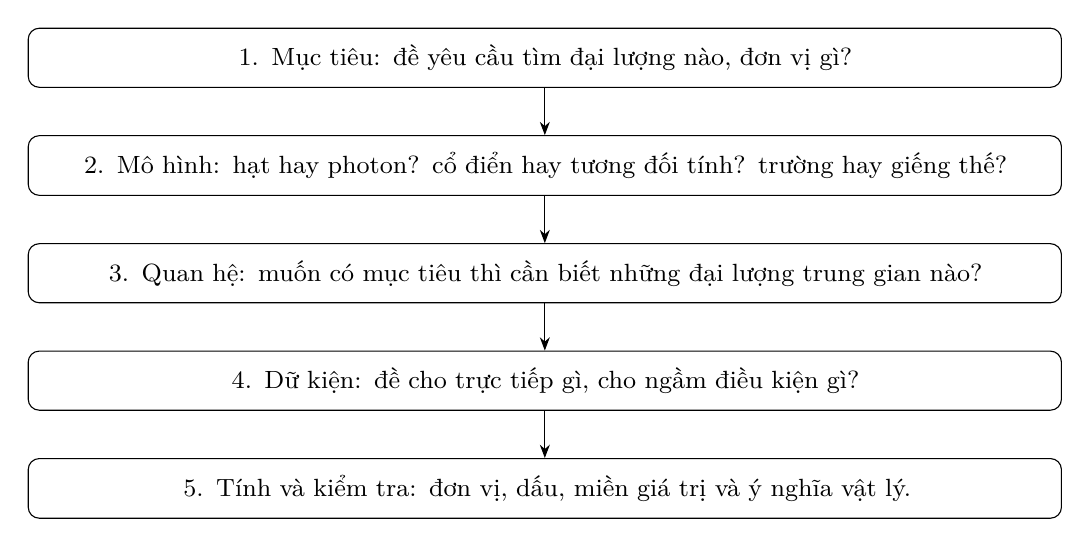
\begin{tikzpicture}[>=Stealth,node distance=6mm,every node/.style={font=\small}]
\node[draw,rounded corners,text width=12.7cm,align=center,inner sep=6pt] (a)
{1. Mục tiêu: đề yêu cầu tìm đại lượng nào, đơn vị gì?};
\node[draw,rounded corners,text width=12.7cm,align=center,inner sep=6pt,below=of a] (b)
{2. Mô hình: hạt hay photon? cổ điển hay tương đối tính? trường hay giếng thế?};
\node[draw,rounded corners,text width=12.7cm,align=center,inner sep=6pt,below=of b] (c)
{3. Quan hệ: muốn có mục tiêu thì cần biết những đại lượng trung gian nào?};
\node[draw,rounded corners,text width=12.7cm,align=center,inner sep=6pt,below=of c] (d)
{4. Dữ kiện: đề cho trực tiếp gì, cho ngầm điều kiện gì?};
\node[draw,rounded corners,text width=12.7cm,align=center,inner sep=6pt,below=of d] (e)
{5. Tính và kiểm tra: đơn vị, dấu, miền giá trị và ý nghĩa vật lý.};
\draw[->] (a)--(b);\draw[->] (b)--(c);\draw[->] (c)--(d);\draw[->] (d)--(e);
\end{tikzpicture}
\end{center}

\textbf{Mẫu ghi đầu bài vào vở}
\begin{itemize}
\item \emph{Tìm:} ký hiệu của đại lượng cần tìm, kèm đơn vị.
\item \emph{Cho:} dữ kiện đã đổi đơn vị; ghi rõ ý nghĩa từng ký hiệu.
\item \emph{Điều kiện:} ban đầu đứng yên, trường đều, góc nhỏ, giếng vô hạn,
hay bỏ qua vận tốc ban đầu, v.v.
\item \emph{Đường giải:} mục tiêu $\leftarrow$ trung gian $\leftarrow$ dữ kiện.
\end{itemize}

Ví dụ muốn tìm bước sóng photon khi electron chuyển mức:
\[
\lambda\ \longleftarrow\ E_\gamma=|E_i-E_f|
\ \longleftarrow\ E_i,E_f
\ \longleftarrow\ \text{mô hình mức năng lượng và các số lượng tử.}
\]
Chỉ khi biết hệ là nguyên tử hydro hay giếng thế, bạn mới chọn được
công thức $E_n$. Không thể dùng một công thức mức năng lượng cho mọi hệ.

\subsection{Các từ đề bài thường dùng để cho điều kiện ngầm}
\begin{tabularx}{\textwidth}{@{}Q{3.6cm}Y@{}}
\toprule
\textbf{Cụm từ trong đề} & \textbf{Dịch thành điều kiện hoặc thao tác}\\\midrule
Ban đầu đứng yên & $v_0=0$, $p_0=0$; năng lượng toàn phần của hạt có khối lượng vẫn là $mc^2$.\\
Được tăng tốc qua $U$ & Độ tăng động năng bằng công của điện trường; với electron và $U$ là độ lớn thế tăng tốc: $\Delta K=eU$.\\
Đều / không đổi & Đại lượng được nêu không thay đổi trong miền đang xét; cần phân biệt không đổi theo không gian với không đổi theo thời gian.\\
Vuông góc / song song & Tách vectơ thành thành phần; lực từ dùng $v_\perp$, chuyển động dọc từ trường dùng $v_\parallel$.\\
Cực đại / cực tiểu & Tìm điều kiện biên hoặc trạng thái thấp nhất; không nhất thiết phải lấy đạo hàm.\\
Chứng minh & Lập quan hệ bằng ký hiệu và giải thích điều kiện; kết quả số riêng lẻ chưa đủ.\\
Đánh giá / ước lượng & Tìm bậc độ lớn bằng gần đúng có giải thích, không mặc nhiên là nghiệm chính xác.\\
Giả thiết / coi như & Là quy tắc của mô hình bài toán. Ví dụ bài 2-8 cố ý thay giá trị $h$.\\
Phát ra một photon & Hệ mất năng lượng: $E_\gamma=E_i-E_f>0$.\\
Hấp thụ một photon & Hệ nhận năng lượng: $E_\gamma=E_f-E_i>0$.\\
\bottomrule
\end{tabularx}

\subsection{Bốn phép kiểm tra sau khi tính}
\begin{enumerate}
\item \textbf{Đơn vị:} vận tốc phải ra m/s, tiêu cự ra m, xác suất không có đơn vị.
\item \textbf{Miền giá trị:} $0\le P\le1$, vận tốc hạt có khối lượng $v<c$,
bước sóng $\lambda>0$; số lượng tử phải thuộc tập cho phép.
\item \textbf{Xu hướng:} giếng hẹp hơn thì năng lượng cao hơn; rào dày hơn
thì khó xuyên qua hơn; tăng thế gia tốc thì chùm khó bị làm lệch hơn.
\item \textbf{Giới hạn:} nếu tắt trường làm lệch thì độ lệch phải về 0;
photon phát xạ phải lấy năng lượng từ hệ.
\end{enumerate}

\chap{Đọc ký hiệu, đơn vị và năng lượng}
\subsection{Một chữ có thể mang nhiều nghĩa}\label{sec:symbol}
Ký hiệu không có nghĩa cố định ở mọi bài. Hãy đọc định nghĩa gần công thức
và dùng đơn vị để nhận diện. Đặc biệt, chữ $E$ có thể vừa là điện trường
vừa là năng lượng trong cùng một tài liệu.

\begin{tabularx}{\textwidth}{@{}Q{2.5cm}Q{4.1cm}Y@{}}
\toprule
\textbf{Ký hiệu} & \textbf{Nghĩa thường gặp} & \textbf{Cách phân biệt}\\\midrule
$e$, $q$ & $e>0$: độ lớn điện tích electron; $q$: điện tích có dấu & Electron có $q=-e$; proton có $q=+e$.\\
$\vec E$, $E$ & Điện trường hoặc năng lượng & Điện trường: V/m hay N/C; năng lượng: J hay eV.\\
$U$, $\varphi$, $V$ & Điện thế, hiệu điện thế, công thoát hoặc thế năng & Điện thế: V; công thoát và thế năng: J hay eV. $\varphi$ cũng có thể là góc hoặc pha.\\
$T$, $K$, $W_{\rm đ}$ & Động năng; $T$ còn là chu kỳ & Động năng có đơn vị J/eV; chu kỳ có đơn vị s.\\
$I$, $P$ & Dòng điện, cường độ bức xạ; công suất hoặc xác suất & A; W/m$^2$; W; xác suất không đơn vị.\\
$p$, $\vec p$, $p_x$ & Động lượng, vectơ động lượng, hình chiếu lên $Ox$ & $p=|\vec p|\ge0$; $p_x$ có thể âm.\\
$L$, $l$, $\ell$ & Chiều dài, số lượng tử hoặc mômen động lượng & Xem ngữ cảnh và đơn vị; dùng $\ell$ cho số lượng tử quỹ đạo trong sổ tay này.\\
$\mu$, $\mu_B$, $\mu_0$ & Mômen từ, magneton Bohr, độ từ thẩm chân không & $\mu_B$: J/T; $\mu_0$: H/m; không thay lẫn nhau.\\
$\nu$, $v$, $\omega$ & Tần số, vận tốc, tần số góc & $\nu$: Hz; $v$: m/s; $\omega=2\pi\nu$: rad/s.\\
$n$ & Số lượng tử, bậc nhiễu xạ, chiết suất hoặc nồng độ & Mỗi công thức phải định nghĩa lại $n$.\\
\bottomrule
\end{tabularx}

\subsection{Những dấu toán học cần đọc được}
\begin{tabularx}{\textwidth}{@{}Q{3cm}Y@{}}
\toprule
\textbf{Dấu} & \textbf{Đọc và hiểu}\\\midrule
$\vec a$, $|\vec a|$ & Vectơ có hướng; độ lớn của vectơ. Biết độ lớn chưa đủ để biết hướng.\\
$\Delta a$ & Độ thay đổi hoặc độ bất định; phải đọc đề để phân biệt.\\
$a'$, $a''$ & Có thể là đạo hàm bậc một, bậc hai; nhưng $\lambda'$ trong Compton là bước sóng sau tán xạ.\\
$\hat A$ & Toán tử: một quy tắc tác động lên hàm, không phải một con số thường.\\
$\psi^*$, $|\psi|^2$ & Liên hợp phức; $|\psi|^2=\psi^*\psi$, luôn thực và không âm.\\
$\langle A\rangle$ & Giá trị kỳ vọng: trung bình kết quả đo trên nhiều hệ cùng trạng thái.\\
$\propto$, $\approx$, $\ll$ & Tỉ lệ với; gần đúng bằng; nhỏ hơn rất nhiều.\\
$\vec a\cdot\vec b$ & Tích vô hướng: $ab\cos\theta$; kết quả là số.\\
$\vec a\times\vec b$ & Tích có hướng: vectơ vuông góc với cả hai; độ lớn $ab\sin\theta$.\\
$\nabla^2$ & Toán tử Laplace: trong tọa độ Đề-các là tổng các đạo hàm riêng bậc hai theo $x,y,z$.\\
\bottomrule
\end{tabularx}

\subsection{Đơn vị và hằng số dùng xuyên suốt}\label{sec:units}
\[
\begin{gathered}
1\unit{eV}=1{,}602\times10^{-19}\unit{J},\qquad
1\unit{keV}=10^3\unit{eV},\quad 1\unit{MeV}=10^6\unit{eV},\\
1\unit{\mathring A}=10^{-10}\unit m,\quad
1\unit{nm}=10^{-9}\unit m=10\unit{\mathring A},\quad
1\unit{mg}=10^{-6}\unit{kg},\\
e\approx1{,}602\times10^{-19}\unit C,\quad
m_e\approx9{,}109\times10^{-31}\unit{kg},\quad
c\approx2{,}998\times10^8\unit{m/s},\\
h\approx6{,}626\times10^{-34}\unit{J\,s},\quad
\hbar=\frac h{2\pi}\approx1{,}055\times10^{-34}\unit{J\,s},\\
m_ec^2\approx511\unit{keV},\qquad
hc\approx1240\unit{eV\,nm},\qquad
\hbar c\approx197{,}3\unit{eV\,nm},\\
\mu_B=\frac{e\hbar}{2m_e}\approx9{,}274\times10^{-24}\unit{J/T},\qquad
R_H\approx1{,}097\times10^7\unit{m^{-1}}.
\end{gathered}
\]
\textbf{Electronvolt là đơn vị năng lượng.} Một electron tăng tốc từ nghỉ
qua độ lớn hiệu điện thế $100\unit V$ nhận động năng $100\unit{eV}$,
không phải $100\unit J$. Nếu đã dùng eV thì không nhân thêm $e$ một lần nữa.

Hai cách tính hợp lệ:
$E_\gamma(\mathrm{eV})=1240/\lambda(\mathrm{nm})$;
hoặc đổi toàn bộ sang SI rồi tính $E_\gamma=hc/\lambda$ ra J.
Nếu dùng $m$ theo kg và $h$ theo J\,s thì năng lượng trong căn phải theo J.

\subsection{Động năng, thế năng và năng lượng toàn phần}\label{sec:energy}
\idea{Động năng là phần gắn với chuyển động. Thế năng mô tả tương tác
và phụ thuộc mốc chọn. Năng lượng toàn phần tương đối tính còn chứa năng lượng nghỉ.}

Trong cơ học không tương đối tính, với thế năng $V$:
\[
K=\frac12mv^2=\frac{p^2}{2m},\qquad E_{\rm cơ}=K+V.
\]
Với hạt tự do tương đối tính:
\[
\gamma=\frac1{\sqrt{1-v^2/c^2}},\quad
\mathcal E=\gamma mc^2=mc^2+K,\quad p=\gamma mv,
\]
\[
\mathcal E^2=p^2c^2+m^2c^4,\qquad
pc=\sqrt{K(K+2mc^2)},\qquad
v=c\sqrt{1-\left(1+\frac K{mc^2}\right)^{-2}}.
\]
Trong tài liệu cũ, $m_0$ thường là khối lượng nghỉ và $m=\gamma m_0$
được gọi là khối lượng tương đối tính. Sổ tay này giữ $m$ cố định là khối
lượng nghỉ và viết $\gamma$ tường minh.

\readit{Nếu đề nói electron có \emph{động năng} $60\unit{keV}$,
thì $K=60\unit{keV}$ và $\mathcal E=571\unit{keV}$.
Nếu đề nói photon năng lượng $60\unit{keV}$ thì $E_\gamma=pc$;
photon không có năng lượng nghỉ.}

\trap{Không dùng $p=mv$ hoặc $K=mv^2/2$ tùy tiện khi $K$ không còn nhỏ
so với $mc^2$. Với electron, hãy so sánh $K$ với $511\unit{keV}$.
Không có một ngưỡng phần trăm chung cho mọi yêu cầu sai số.}

\chap{Chương 1: hạt tích điện, trường và quang học điện tử}
\subsection{Các bộ phận trong đề đang làm việc gì?}\label{sec:c1words}
\begin{tabularx}{\textwidth}{@{}Q{3.3cm}Y@{}}
\toprule
\textbf{Thuật ngữ} & \textbf{Ý nghĩa và thông tin cần lấy}\\\midrule
Điện tử / electron & Cùng một hạt: điện tích $-e$, khối lượng $m_e$.\\
Chân không & Môi trường rất ít hạt khí; trong bài thường bỏ qua va chạm và lực cản.\\
Catot (K) & Điện cực phát electron; hay được chọn làm mốc điện thế $0$.\\
Anot (A) & Điện cực thu electron hoặc điện cực tăng tốc; xác định vị trí và điện thế trên hình.\\
Lưới tăng tốc (G) & Điện cực cho chùm đi qua; hiệu điện thế tạo động năng cho electron.\\
Diapham / diaphragm & Tấm điện cực có lỗ cho chùm đi qua. Điện trường gần lỗ có thể làm chùm hội tụ hoặc phân kỳ.\\
Bản lái tia & Hai bản điện cực tạo điện trường ngang để bẻ chùm electron.\\
Màn huỳnh quang & Electron đập vào tạo vết sáng; độ lệch $D$ là khoảng cách vết sáng tới vị trí khi chưa lái tia.\\
Ống tia điện tử / dao động ký & Hệ tạo, tăng tốc, làm lệch và quan sát chùm electron.\\
Trục quang học & Trục đối xứng của hệ điện cực; đo khoảng cách và độ lệch theo trục này.\\
Chùm hẹp, gần trục & Các tia gần trục, góc nhỏ: $\sin\theta\approx\tan\theta\approx\theta$ theo radian.\\
\bottomrule
\end{tabularx}

\subsection{Điện thế, điện trường và lực điện}\label{sec:electric}
\idea{Điện thế là một số gắn với mỗi vị trí. Điện trường là một vectơ
cho biết điện tích dương sẽ bị đẩy theo hướng nào. Electron mang điện âm
nên lực điện ngược chiều điện trường.}
\[
\vec E=-\nabla\Phi,\qquad \vec F=q\vec E,\qquad
V_{\rm điện}=q\Phi,\qquad
K_f-K_i=q(\Phi_i-\Phi_f).
\]
Ở đây $\Phi$ là điện thế (V), $V_{\rm điện}$ là thế năng (J).
Giữa hai bản song song cách $d$, bỏ qua hiệu ứng mép,
độ lớn điện trường là $E=|\Delta\Phi|/d$.

Với electron đi từ điện thế thấp lên cao một lượng $U>0$:
$\Delta K=eU$. Nếu xuất phát gần như đứng yên và không tương đối tính:
\[
\frac12m_ev^2=eU\quad\Rightarrow\quad v=\sqrt{\frac{2eU}{m_e}}.
\]
\think{Muốn có $v$ sau tăng tốc, cần $K$; muốn có $K$, cần công điện trường
và động năng ban đầu. Không cần giải quỹ đạo nếu đề chỉ hỏi độ lớn vận tốc.}

\trap{Electron có thể đi về phía điện thế cao trong khi thế năng giảm,
vì $V_{\rm điện}=-e\Phi$. Từ trường tĩnh riêng lẻ không làm đổi động năng;
điện trường có thể làm đổi động năng.}

\subsection{Lái tia tĩnh điện và độ nhạy: bài 1-1}\label{sec:crt}
\idea{Độ nhạy cho biết tăng một đơn vị tín hiệu điều khiển thì vết sáng
dịch bao nhiêu. Đây là tỉ số giữa kết quả và tín hiệu gây ra kết quả.}
Gọi $U_0$ là thế tăng tốc, $U_k$ là độ lớn điện áp giữa bản lái tia,
$l$ là chiều dài bản, $d$ là khe bản. Gọi $l_2$ là khoảng cách từ mép ra
đến màn và $L=l/2+l_2$ là khoảng cách từ \emph{giữa bản} đến màn.

\begin{center}
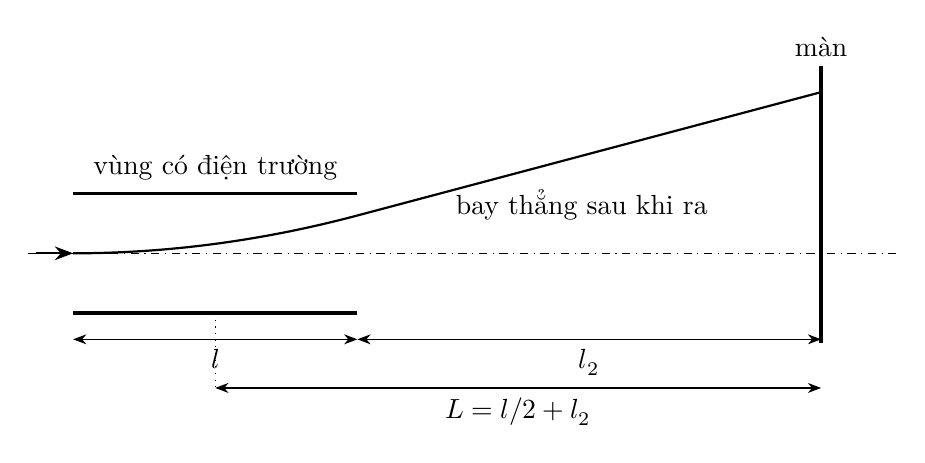
\begin{tikzpicture}[>=Stealth,scale=0.95]
\draw[dashdotted] (-0.6,0)--(11,0);
\draw[very thick] (0,0.8)--(3.8,0.8);
\draw[very thick] (0,-0.8)--(3.8,-0.8);
\draw[very thick] (10,-1.2)--(10,2.5);
\node[above] at (10,2.5) {màn};
\draw[->,thick] (-0.5,0)--(0,0);
\draw[thick,domain=0:3.8,samples=50] plot (\x,{0.035*\x*\x});
\draw[thick] (3.8,0.5054)--(10,2.1546);
\draw[<->] (0,-1.15)--(3.8,-1.15) node[midway,below] {$l$};
\draw[<->] (3.8,-1.15)--(10,-1.15) node[midway,below] {$l_2$};
\draw[dotted] (1.9,-0.8)--(1.9,-1.85);
\draw[<->] (1.9,-1.8)--(10,-1.8) node[midway,below] {$L=l/2+l_2$};
\node at (1.9,1.15) {vùng có điện trường};
\node at (6.8,0.65) {bay thẳng sau khi ra};
\end{tikzpicture}
\end{center}

Theo độ lớn, trong gần đúng góc nhỏ:
\[
v_x\approx\sqrt{\frac{2eU_0}{m_e}},\quad
a_y=\frac{eU_k}{m_ed},\quad t_1=\frac l{v_x}.
\]
Lệch trong bản: $y_1=a_yt_1^2/2$. Ra khỏi bản, electron đã có
$v_y=a_yt_1$, nên còn lệch thêm $v_yl_2/v_x$ trước khi chạm màn.
\[
|D|=\frac{U_klL}{2dU_0},\qquad
S_E=\frac{|D|}{U_k}=\frac{lL}{2dU_0}.
\]
\think{$S_E\leftarrow D/U_k\leftarrow$ lệch trong bản + lệch khi bay ra màn
$\leftarrow a_y,t_1,v_x$. Đây là lý do xuất hiện khoảng cách từ giữa bản đến màn.}

\ex{bài 1-1}
\textbf{Tìm:} $S_E$ (m/V). \textbf{Cho:}
$U_0=900\unit V$, $L=0{,}20\unit m$, $l=0{,}020\unit m$, $d=0{,}005\unit m$.
\[
S_E=\frac{0{,}020\times0{,}20}{2\times0{,}005\times900}
\approx4{,}44\times10^{-4}\unit{m/V}=0{,}444\unit{mm/V}.
\]
Đề không cho $U_k$ vẫn tìm được độ nhạy, vì $U_k$ đã triệt tiêu.
Tăng $U_0$ làm electron bay nhanh hơn và ít lệch hơn: $S_E$ giảm.

\subsection{Từ trường: tròn, xoắn ốc và lái tia bằng cuộn dây}\label{sec:magnetic}
\idea{Lực từ luôn vuông góc vận tốc, nên bẻ hướng chuyển động.
Nếu có cả thành phần vận tốc dọc từ trường, hạt vừa quay tròn vừa tiến dọc trục.}
\[
\vec F=q\vec v\times\vec B,\quad |F|=|q|vB\sin\alpha,
\qquad v_\perp=v\sin\alpha,\quad v_\parallel=v\cos\alpha.
\]
Với chuyển động không tương đối tính:
\[
r=\frac{mv_\perp}{|q|B},\quad
\omega_c=\frac{|q|B}{m},\quad
\tau_c=\frac{2\pi m}{|q|B},\quad
b=v_\parallel\tau_c.
\]
$r$ là bán kính xoắn ốc, $b$ là \emph{bước xoắn}: độ tiến dọc trục trong một vòng.
Nếu $v_\parallel=0$ thì quỹ đạo tròn; nếu $v_\perp=0$ thì hạt đi thẳng.
Khi cần tương đối tính, dùng $r=p_\perp/(|q|B)$ và
$\tau_c=2\pi\gamma m/(|q|B)$.

\textbf{Bài 1-2:} cuộn dây tạo $B$ tỉ lệ dòng điện $I$; trong vùng từ trường
hẹp dài $l$, góc lệch nhỏ $\theta\approx l/r$.
Với $L$ từ tâm vùng làm lệch đến màn:
\[
|D|\approx L\theta=\frac{eBlL}{m_ev},\qquad
S_I=\frac{|D|}{I}=\frac{elL}{m_ev}\frac BI.
\]
\think{$S_I\leftarrow D/I\leftarrow$ hình học tia và $r$
$\leftarrow v,B/I\leftarrow U_0$, kích thước và số vòng cuộn dây.}

\textbf{Cuộn dây Helmholtz và số vòng.}
Với hai cuộn tròn cùng bán kính $R$, mỗi cuộn $N$ vòng,
tâm mỗi cuộn cách trung điểm $z$, từ trường tại trung điểm là
\[
B=\frac{\mu_0NI R^2}{(R^2+z^2)^{3/2}}.
\]
Nếu đề gọi $W=2N$ là tổng số vòng, công thức thành
$B=\mu_0 IW R^2/[2(R^2+z^2)^{3/2}]$.
Hình học Helmholtz chuẩn có khoảng cách hai cuộn bằng $R$, tức $2z=R$.
\textbf{Bài 1-2 cho $2z=5\unit{cm}$ và $R=2{,}5\unit{cm}$: dùng đúng hình học
và công thức tổng quát đề cho}, không tự thay công thức Helmholtz chuẩn.

\trap{Hướng $\vec v\times\vec B$ là hướng lực của điện tích dương;
electron bị lực theo hướng ngược lại. $B$ (T) và $H$ (A/m) khác nhau;
trong chân không $B=\mu_0H$.}

\subsection{Quang học điện tử, lưới cầu và tiêu cự}\label{sec:lens}
\idea{Thấu kính điện tử là vùng trường làm thay đổi hướng chùm hạt.
Chùm hội tụ tiến về trục; chùm phân kỳ tách xa trục.
Tiêu điểm là nơi chùm tới song song gặp trục sau thấu kính hội tụ.}

\textbf{Mặt đẳng thế} là mặt mà điện thế có cùng giá trị.
\textbf{Pháp tuyến} là đường vuông góc với mặt tại điểm xét;
với mặt cầu, pháp tuyến đi qua tâm cầu.
\textbf{Góc tới và góc khúc xạ} đo so với pháp tuyến, không đo so với mặt.

Trong mô hình electron không tương đối tính đi qua lớp chuyển thế mỏng,
động lượng tiếp tuyến được bảo toàn:
\[
p_1\sin\alpha=p_2\sin\beta,\qquad
\frac{\sin\alpha}{\sin\beta}=\frac{p_2}{p_1}
=\sqrt{\frac{U_2}{U_1}}.
\]
Ở đây $U_i>0$ là điện thế gia tốc tính từ cùng mốc catot,
khi động năng ban đầu được bỏ qua. Không dùng tỉ số hai điện thế
với mốc chọn tùy ý; bản chất là tỉ số động lượng.

\readit{Bài 1-3 cho hai lưới cầu đồng tâm. Hãy vẽ pháp tuyến đi qua tâm,
rồi mới so sánh góc tới, góc khúc xạ. Với chiều cong như hình đề và
$U_2>U_1$, tia lệch về pháp tuyến và hướng vào trục.}
Ở gần trục, gọi $y$ là độ cao tia và $R$ là bán kính cầu:
\[
\alpha\approx y/R,\quad
\beta\approx\sqrt{U_1/U_2}\,\alpha,\quad
\delta=\alpha-\beta,\quad
f\approx\frac y\delta=\frac R{1-\sqrt{U_1/U_2}}.
\]
\think{$f\leftarrow y/\delta\leftarrow$ góc bẻ tia
$\leftarrow$ khúc xạ + pháp tuyến mặt cầu. Muốn chứng minh hội tụ,
cần chỉ ra tia bẻ vào trục và $f$ không phụ thuộc độ cao $y$ trong gần đúng này.}

\subsection{Diapham và hệ hai thấu kính: bài 1-4, 1-5}\label{sec:diaphragm}
Một lỗ tròn trên điện cực có thể hoạt động như thấu kính mỏng vì trường
gần lỗ có thành phần ngang. \emph{Mỏng} nghĩa là vùng tác dụng ngắn;
\emph{gần trục} nghĩa là các tia chỉ tạo góc nhỏ với trục.

Để tránh nhầm dấu, gọi $g_1=d\Phi/dz$ và $g_2=d\Phi/dz$ là
\textbf{độ dốc điện thế} ngay trước và sau diapham. Trong mô hình đang dùng:
\[
\frac1f=\frac{g_2-g_1}{4U_D},\qquad
g_1\approx\frac{U_D-U_G}{d_1},\qquad
g_2\approx\frac{U_A-U_D}{d_2}.
\]
$U_D$ là điện thế diapham so với catot; $d_1,d_2$ là chiều dài hai miền.
Điện trường vật lý có hình chiếu $E_z=-g$. Vì vậy, nếu ký hiệu $E_1,E_2$
trong một lời giải thực chất chỉ độ dốc điện thế, đừng trộn chúng với
$E_z$ rồi giữ nguyên dấu công thức.

\ex{bài 1-4}
\textbf{Câu chữ quan trọng:} anot nối với diapham $\Rightarrow U_A=U_D$
$\Rightarrow g_2=0$. Chùm tới song song hội tụ tại anot
$\Rightarrow f=d_2$.
\[
\underbrace{d_2}_{\text{vị trí phải hội tụ}}
=\underbrace{\frac{4U_Dd_1}{U_G-U_D}}_{\text{tiêu cự do điện thế tạo ra}}
\quad\Rightarrow\quad
U_D=\frac{d_2U_G}{4d_1+d_2}.
\]
Thay $d_1=0{,}5\unit{cm}$, $d_2=0{,}8\unit{cm}$,
$U_G=200\unit V$ được $U_D\approx57{,}1\unit V$.
Tỉ số chiều dài cho phép dùng cùng đơn vị cm trong phép tính này.

\textbf{Bài 1-5: làm lần lượt từng thấu kính.}
Gọi khoảng cách hai thấu kính là $d$, ảnh do thấu kính đầu cách nó
$b_1=f_1$ vì chùm đầu song song. Với quy ước thấu kính mỏng:
\[
\frac1{a_2}+\frac1{b_2}=\frac1{f_2},\qquad
a_2=d-f_1.
\]
Nếu anot cách thấu kính thứ hai $d$, đặt $b_2=d$.
$a_2<0$ có nghĩa là vật ảo đối với thấu kính thứ hai; không được tự đổi thành
giá trị dương. Mỗi $f_i$ phải được viết theo các điện thế trước khi giải điều kiện hội tụ.

\think{$U_2\leftarrow$ điều kiện ảnh nằm trên anot
$\leftarrow f_1(U_2),f_2(U_2)$ và khoảng cách
$\leftarrow$ độ dốc điện thế hai phía từng diapham.}

\subsection{Thấu kính từ: khái niệm lý thuyết cần nhận ra}\label{sec:maglens}
\idea{Cuộn dây ngắn tạo từ trường đối xứng trục, không đều.
Electron bị cuốn quay và có lực hướng vào trục, nên chùm có thể hội tụ.}
Trong mô hình thấu kính từ mỏng, yếu, không tương đối tính, với thế tăng tốc
$U_0$ gần như không đổi:
\[
\frac1f=\frac{e}{8m_eU_0}\int_{-\infty}^{+\infty}B_z^2(z)\,dz.
\]
$B_z$ là thành phần từ trường dọc trục. Hệ số $e/m_e$ cần có để đúng đơn vị.
Vì tích phân $B_z^2$ không âm, thấu kính từ kiểu này có tác dụng hội tụ.
Đổi chiều dòng cuộn dây đảo chiều quay ảnh nhưng không đổi dấu $1/f$.

\readit{Nếu đề chỉ hỏi nguyên lý, cần nói rõ: trường không đều tạo chuyển động
quay và tác dụng hội tụ; từ trường tĩnh không cấp thêm động năng.
Không đồng nhất thấu kính từ với vùng từ trường đều dùng để lái lệch chùm.}

\chap{Chương 2: photon, sóng vật chất và cơ học lượng tử}
\subsection{Photon, bức xạ và thông lượng}\label{sec:photon}
\idea{Photon là lượng tử của bức xạ điện từ. Ánh sáng truyền năng lượng
bằng các lượng $h\nu$. Cường độ bức xạ cho biết tổng năng lượng tới một diện
tích trong một giây; năng lượng photon cho biết phần của một photon.}
\[
E_\gamma=h\nu=\hbar\omega=\frac{hc}{\lambda},\quad
p_\gamma=\frac{E_\gamma}{c}=\frac h\lambda,\quad
c=\lambda\nu.
\]
$\lambda$ là bước sóng trong chân không; $\nu$ là tần số;
$\omega=2\pi\nu$. Photon có khối lượng nghỉ bằng 0 nhưng có động lượng.

Nếu nguồn phát đều mọi hướng, công suất bức xạ $P_{\rm bx}$ trải trên
mặt cầu bán kính $r$:
\[
I_{\rm bx}=\frac{P_{\rm bx}}{4\pi r^2},\qquad
\Phi_\gamma=\frac{I_{\rm bx}}{E_\gamma}.
\]
$I_{\rm bx}$: W/m$^2$; $\Phi_\gamma$: số photon/(m$^2$\,s).
Với diện tích nhận $S$ đặt vuông góc tia và thời gian $t$,
số photon tới là $N_\gamma=\Phi_\gamma St$.

\readit{Bài 2-1 nói \emph{công suất bức xạ bằng 5\% công suất định mức}:
$P_{\rm bx}=0{,}05P$. Nguyên tử coi như đĩa đường kính $d$:
diện tích hứng $S_a=\pi d^2/4$, không phải diện tích cả mặt cầu.}
Theo mô hình tích lũy năng lượng liên tục mà bài yêu cầu kiểm tra:
\[
P_a=I_{\rm bx}S_a,\qquad t=\frac{\varphi}{P_a}.
\]
Với dữ kiện bài 2-1, $t\approx58\unit s$, quá dài so với sự phát electron
gần như tức thời quan sát trong quang điện. Đây là mục đích của bài:
nhận ra giới hạn của mô hình sóng cổ điển trong cách giải thích hiện tượng.

\subsection{Quang điện: công thoát, ngưỡng và thế hãm}\label{sec:photoelectric}
\idea{Electron trong kim loại cần nhận ít nhất một năng lượng để thoát ra.
Phần photon còn dư sau khi trả năng lượng thoát trở thành động năng electron.}
\textbf{Công thoát} $\varphi$ (cũng viết $W_0,A$) là năng lượng nhỏ nhất cần
để đưa electron ra khỏi bề mặt vật liệu theo mô hình quang điện.
\[
K_{\max}=h\nu-\varphi=\frac{hc}{\lambda}-\varphi.
\]
\textbf{Giới hạn quang điện} là bước sóng dài nhất còn đủ năng lượng:
\[
\lambda_0=\frac{hc}{\varphi},\quad \nu_0=\frac\varphi h,
\qquad \lambda\le\lambda_0\ \Leftrightarrow\ h\nu\ge\varphi.
\]
\textbf{Thế hãm} $U_h\ge0$ là độ lớn điện áp ngược đủ chặn cả electron
nhanh nhất: $eU_h=K_{\max}$.

\ex{bài 2-2}
Đề cho $\lambda=2500\unit{\mathring A}=250\unit{nm}$,
$\varphi=2{,}2\unit{eV}$, $I_{\rm bx}=2\unit{W/m^2}$.
\[
E_\gamma\approx\frac{1240}{250}=4{,}96\unit{eV},\qquad
K_{\max}\approx4{,}96-2{,}2=2{,}76\unit{eV}.
\]
Muốn tìm \emph{số electron do một đơn vị diện tích phát ra trong một đơn vị
thời gian}, trước hết tìm thông lượng photon. Nếu mỗi photon tới làm bật
một electron, tức hiệu suất lượng tử $\eta=1$:
\[
\Phi_e=\eta\frac{I_{\rm bx}}{E_\gamma}
\approx\frac2{4{,}96\times1{,}602\times10^{-19}}
\approx2{,}52\times10^{18}\unit{m^{-2}s^{-1}}.
\]
Đây là giả thiết lý tưởng. Nếu đề cho $\eta$ khác 1, phải nhân thêm $\eta$.
Mật độ dòng điện phát ra là $j=e\Phi_e$ (A/m$^2$).

\think{$K_{\max}\leftarrow E_\gamma-\varphi\leftarrow\lambda,\varphi$;
còn $\Phi_e\leftarrow$ năng lượng tới mỗi giây trên mỗi diện tích chia cho
năng lượng mỗi photon. Hai yêu cầu dùng hai nhánh suy luận khác nhau.}

\trap{Tăng cường độ ở cùng tần số làm tăng số photon tới, không làm tăng
năng lượng của từng photon. Nếu dưới ngưỡng, phép trừ ra số âm chỉ báo
\emph{không xảy ra quang điện trong mô hình một photon}, không phải động năng âm.}

\subsection{Compton: tán xạ và electron giật lùi}\label{sec:compton}
\idea{Photon va chạm với electron, đổi hướng và truyền một phần năng lượng,
động lượng cho electron. Electron nhận động năng nên photon mất năng lượng
và có bước sóng dài hơn.}
Mô hình Compton cơ bản: electron tự do, ban đầu đứng yên.
Góc $\theta$ là góc giữa hướng photon tới và photon sau tán xạ.
\[
\lambda'-\lambda=\frac{h}{m_ec}(1-\cos\theta),\qquad
\lambda_C=\frac h{m_ec}\approx2{,}426\times10^{-12}\unit m.
\]
Một dạng tiện khi đề cho năng lượng photon:
\[
E_\gamma'=\frac{E_\gamma}{1+\dfrac{E_\gamma}{m_ec^2}(1-\cos\theta)},
\qquad K_e=E_\gamma-E_\gamma'.
\]
Tán xạ ngược nghĩa là $\theta=180^\circ$, nên $1-\cos\theta=2$.
Electron \emph{giật lùi} chỉ electron nhận động lượng sau va chạm;
không có nghĩa nó nhất thiết bay ngược hướng photon ban đầu.

\ex{bài 2-3: photon $0{,}3\unit{MeV}$ tán xạ ngược}
\textbf{Tìm:} $v_e$. Hãy suy ngược:
\[
v_e\ \longleftarrow\ K_e\ \longleftarrow\ E_\gamma'
\ \longleftarrow\ E_\gamma,\theta.
\]
Dùng $m_ec^2=0{,}511\unit{MeV}$:
\[
E_\gamma'\approx\frac{0{,}3}{1+2(0{,}3/0{,}511)}
\approx0{,}138\unit{MeV},\quad K_e\approx0{,}162\unit{MeV}.
\]
\[
\gamma_e=1+\frac{K_e}{m_ec^2}\approx1{,}317,
\qquad v_e=c\sqrt{1-\gamma_e^{-2}}\approx0{,}651c.
\]
Nếu đề yêu cầu \emph{áp dụng bảo toàn rồi kiểm tra bằng Compton},
phải xuất phát từ hai phương trình sau, không chỉ thay công thức Compton:
\[
E_\gamma+m_ec^2=E_\gamma'+\mathcal E_e,\qquad
\frac{E_\gamma}{c}=-\frac{E_\gamma'}{c}+p_e.
\]
Kết hợp $\mathcal E_e^2=p_e^2c^2+m_e^2c^4$ để tìm $E_\gamma'$.
Dấu trừ trong phương trình động lượng là do photon bật ngược.

\subsection{Sóng de Broglie: bước sóng của hạt}\label{sec:debroglie}
\idea{Hạt vật chất có thể tạo hiện tượng giao thoa và nhiễu xạ.
Bước sóng de Broglie nối đại lượng sóng $\lambda$ với động lượng hạt $p$.}
\[
\lambda=\frac hp.
\]
Đây là quan hệ chung; chỉ bước chuyển từ năng lượng sang $p$ mới thay đổi:
\[
\begin{array}{ll}
\text{Không tương đối tính:}&p=\sqrt{2mK},\quad \lambda=h/\sqrt{2mK};\\[4pt]
\text{Tương đối tính:}&pc=\sqrt{K(K+2mc^2)},\quad
\lambda=hc/\sqrt{K(K+2mc^2)}.
\end{array}
\]
Với electron tăng tốc từ nghỉ qua $U$, đặt $K=eU$.
Gần đúng không tương đối tính cho
$\lambda(\mathrm{\mathring A})\approx12{,}27/\sqrt{U(\mathrm V)}$.
Ví dụ bài 2-4 cho $\lambda=1\unit{\mathring A}$:
$U\approx(12{,}27)^2\unit V\approx150\unit V$.

\readit{\emph{Bước sóng kết hợp}, \emph{bước sóng liên kết} và
\emph{bước sóng de Broglie} đều chỉ $h/p$ trong các bài này.
\emph{Hạt siêu tương đối tính} có $\mathcal E\gg mc^2$:
$pc\approx\mathcal E$, nên $\lambda\approx hc/\mathcal E$,
gần bước sóng photon cùng năng lượng. Đây là ý tưởng bài 2-5.}

\trap{Electron và photon cùng bước sóng thì cùng \emph{độ lớn động lượng},
nhưng không có cùng vận tốc hay cùng quan hệ năng lượng.
$c=\lambda\nu$ không phải công thức chung cho sóng vật chất.}

\subsection{Nhiễu xạ, giao thoa và góc trên hình}\label{sec:diffraction}
\textbf{Giao thoa} là sự cộng các biên độ sóng tạo vùng tăng cường, triệt tiêu.
\textbf{Vân} là các vùng cực đại hoặc cực tiểu trên màn.
\textbf{Nhiễu xạ} là biểu hiện lan, đổi phân bố sóng khi gặp khe hoặc cấu trúc;
tinh thể tạo các cực đại do sự giao thoa của các sóng tán xạ.

\textbf{Hai khe Young: bài 2-8.} Nếu hai khe cách nhau $d$, màn cách $L$
và các góc nhỏ, khoảng cách hai vân sáng kề nhau là
\[
i=\frac{\lambda L}{d}=\frac{hL}{mvd}.
\]
Muốn tìm $i$, cần $\lambda$; muốn có $\lambda$, cần động lượng.
Bài 2-8 cố ý cho $h$ rất lớn: giữ nguyên $h$ trong đề, không sửa về hằng số thực.

\textbf{Bragg: bài 2-7.} Các mặt phẳng mạng tinh thể cách nhau $d$;
góc trượt $\theta$ là góc giữa tia và mặt phẳng mạng.
Điều kiện cực đại bậc $n$:
\[
2d\sin\theta=n\lambda.
\]
\emph{Bậc nhất} nghĩa là $n=1$.
Góc giữa tia tới và tia nhiễu xạ trong hình học truyền qua tương ứng là $2\theta$.
Nếu màn cách màng $L$, bán kính vòng nhiễu xạ:
\[
r=L\tan(2\theta)\approx2L\theta\approx\frac{nL\lambda}{d}.
\]
\think{$r\leftarrow2\theta\leftarrow\lambda,d,n
\leftarrow$ động lượng electron và động năng đề cho. Với $K=60\unit{keV}$,
dùng quan hệ tương đối tính để tính $\lambda$ nếu cần kết quả chính xác hơn.}

\trap{Không lấy $r=L\tan\theta$ khi $\theta$ đang là góc Bragg.
\emph{Khoảng cách mặt mạng} là khoảng cách các mặt tinh thể đang gây phản xạ;
không tự đổi thành một hằng số mạng khác nếu đề đã cho $d$.}

\subsection{Hàm sóng phẳng, pha và vận tốc nhóm}\label{sec:phase}
Một sóng phẳng có thể viết
\[
\Psi(x,t)=A e^{i(kx-\omega t)},\qquad
k=\frac{2\pi}{\lambda},\quad p=\hbar k,\quad E=\hbar\omega.
\]
$i^2=-1$ là đơn vị ảo; $A$ là biên độ; $kx-\omega t$ là pha;
$k$ là số sóng góc (m$^{-1}$). \emph{Đơn sắc} nghĩa là có một tần số.
\emph{Sóng phẳng} có các mặt cùng pha là mặt phẳng.
Hàm phức là công cụ biểu diễn; xác suất lấy từ môđun bình phương.

\textbf{Gói sóng / nhóm sóng} là tổng của nhiều sóng có số sóng gần nhau,
có thể tạo một vùng tập trung trong không gian.
\[
v_{\rm pha}=\frac\omega k=\frac Ep,\qquad
v_{\rm nhóm}=\frac{d\omega}{dk}=\frac{dE}{dp}.
\]
Nếu $E=\mathcal E=\sqrt{p^2c^2+m^2c^4}$ là năng lượng toàn phần:
\[
v_{\rm pha}=\frac{c^2}{v},\qquad v_{\rm nhóm}=v.
\]
Nếu đã bỏ pha năng lượng nghỉ trong mô hình Schrödinger tự do,
dùng $E=K=p^2/(2m)$ thì $v_{\rm pha}=v/2$, vẫn có $v_{\rm nhóm}=v$.
Hai biểu thức vận tốc pha dùng hai quy ước năng lượng khác nhau.

\readit{Với bài 2-6, trước khi tính $E/p$, hãy nói rõ $E$ đang là
năng lượng toàn phần hay động năng. Slide dùng $c^2/v$ khi giữ năng lượng nghỉ.
Vận tốc pha lớn hơn $c$ ở đây không phải vận tốc truyền tín hiệu.}

\subsection{Hàm sóng, xác suất và chuẩn hóa}\label{sec:wavefunction}
\idea{Hàm sóng mô tả trạng thái lượng tử. Từ nó, ta tính phân bố kết quả đo.
Trong một chiều, $|\psi(x)|^2$ là mật độ xác suất theo vị trí.}
\[
P(a\le x\le b)=\int_a^b|\psi(x)|^2\,dx,\qquad
\int_{\text{toàn miền}}|\psi(x)|^2\,dx=1.
\]
\textbf{Chuẩn hóa} là chọn hệ số để tổng xác suất bằng 1.
Trong một chiều, $|\psi|^2$ có đơn vị m$^{-1}$ và $\psi$ có đơn vị m$^{-1/2}$.
Mật độ có thể lớn hơn $1\unit{m^{-1}}$; xác suất tích phân mới phải nằm từ 0 đến 1.
Với phân bố liên tục, xác suất tại đúng một điểm đơn lẻ bằng 0;
ý nghĩa thực tế là xác suất trong một khoảng nhỏ $dx$.

\think{Đề cho $\psi(x)=Af(x)$ và hỏi $A$:
$A\leftarrow |A|^2\int|f|^2dx=1$. Đề hỏi xác suất:
chuẩn hóa trước nếu cần, rồi tích phân trên đúng khoảng đề hỏi.}

\ex{bài 2-17: chuẩn hóa hàm sin trong giếng}
Với $\psi_n(x)=A\sin(n\pi x/L)$ trên $0<x<L$:
\[
1=|A|^2\int_0^L\sin^2\left(\frac{n\pi x}{L}\right)dx
=|A|^2\frac L2
\quad\Rightarrow\quad A=\sqrt{\frac2L}.
\]
Ta chọn $A$ thực dương cho tiện. Một pha chung $e^{i\alpha}$ không làm
đổi $|\psi|^2$. Đồng nhất thức cần dùng:
$\sin^2u=(1-\cos2u)/2$.

\trap{Nếu $\psi$ phức, dùng $\psi^*\psi$, không dùng $\psi^2$.
Chỉ việc thỏa phương trình Schrödinger chưa đảm bảo hàm đã chuẩn hóa;
phương trình là tuyến tính nên nhân với hằng số vẫn là nghiệm.}

\subsection{Bất định vị trí và động lượng}\label{sec:uncertainty}
\idea{Một trạng thái có phân bố vị trí rất hẹp thì không thể đồng thời có
phân bố động lượng hẹp tùy ý. Độ bất định ở đây là độ trải của kết quả đo,
không đơn thuần là sai số dụng cụ.}
Với $\sigma_x,\sigma_p$ là độ lệch chuẩn:
\[
\sigma_x\sigma_{p_x}\ge\frac\hbar2=\frac h{4\pi}.
\]
Slide Chương II hiện có cũng ghi dạng $h/(4\pi)$.
Một số đề và lời giải cũ trong thư mục dùng $\Delta x\Delta p\gtrsim\hbar$
để ước lượng hoặc quy ước $\Delta$ khác. \textbf{Hai hệ số không được coi là
hai bất đẳng thức chính xác tương đương.}
Khi đề chỉ định hệ thức, ghi rõ và dùng hệ thức đó. Khi nói độ lệch chuẩn
và không có quy ước riêng, dùng $\hbar/2$.

\textbf{Độ bất định tương đối} $\delta=\Delta p/p$ là một tỉ số.
\emph{Đo đến phần nghìn} trong bài 2-9 cho $\delta=10^{-3}$:
$\Delta p=10^{-3}p$, không phải $\Delta p=10^{-3}\unit{kg\,m/s}$.

\think{$\Delta x_{\min}\leftarrow C/\Delta p
\leftarrow\delta p\leftarrow m,v$;
với $C=\hbar/2$ nếu $\Delta$ là độ lệch chuẩn, hoặc $C$ do đề chỉ định.}
Với electron $v=1{,}8\times10^8\unit{m/s}\approx0{,}6c$,
phải tính $p=\gamma m_ev$, $\gamma\approx1{,}25$.
Theo hằng số làm tròn, $p\approx2{,}05\times10^{-22}\unit{kg\,m/s}$,
$\Delta p\approx2{,}05\times10^{-25}\unit{kg\,m/s}$.
Khi $C=\hbar/2$, $\Delta x_{\min}\approx2{,}58\unit{\mathring A}$;
khi dùng $C=\hbar$, kết quả gấp đôi, khoảng $5{,}15\unit{\mathring A}$.

\textbf{Bài 2-11:} nếu $\Delta p=p=h/\lambda$ thì
$\Delta x_{\min}=C\lambda/h$.
Dạng chuẩn cho $\lambda/(4\pi)$; quy ước $C=\hbar$ cho $\lambda/(2\pi)$.

\subsection{Độ rộng vạch và thời gian sống}\label{sec:lifetime}
\textbf{Vạch quang phổ} là một vùng bước sóng hoặc tần số hẹp ứng với
chuyển mức. \textbf{Độ rộng vạch} là độ trải của vùng đó.
\textbf{Thời gian sống} $\tau$ đặc trưng thời gian hệ tồn tại trong trạng thái kích thích.
Trạng thái sống ngắn thường tạo vạch có độ rộng tự nhiên lớn hơn.

Với $E_\gamma=hc/\lambda$ và độ rộng nhỏ so với $\lambda$:
\[
|\Delta E|\approx\frac{hc}{\lambda^2}|\Delta\lambda|.
\]
Với sự suy giảm xác suất theo hàm mũ, độ rộng năng lượng tự nhiên
\emph{toàn phần tại nửa cực đại} (FWHM) là $\Gamma=\hbar/\tau$.
Khi $\Delta\lambda$ biểu thị độ rộng tương ứng:
\[
\tau\approx\frac\hbar\Gamma
\approx\frac{\lambda^2}{2\pi c\,\Delta\lambda}.
\]
FWHM nghĩa là khoảng cách hai điểm mà cường độ còn nửa giá trị đỉnh.
Nếu đề dùng hệ thức bất định năng lượng-thời gian với quy ước khác,
hệ số có thể khác. Quan hệ năng lượng-thời gian không hoàn toàn giống
cặp toán tử vị trí-động lượng; phải hiểu $\Delta t$ trong bài đang chỉ gì.

\readit{Bài 2-10 trong \texttt{baitap.tex} cho
$\lambda=4000\unit{\mathring A}$ và $\Delta\lambda=10^{-4}\unit{\mathring A}$.
Với quy ước độ rộng tự nhiên FWHM, $\tau\approx8{,}5\times10^{-9}\unit s$.
Bản lời giải biên soạn lại ghi bộ dữ kiện khác; cần quay lại đúng đề.
Không trộn dữ kiện của hai bản.}

\textbf{Bài 2-12:} trong mô hình không tương đối tính,
$K=p^2/(2m)$ nên với biến thiên nhỏ $\Delta K\approx v\Delta p$.
Đề định nghĩa $\Delta t=\Delta x/v$, do đó
$\Delta K\Delta t\approx\Delta p\Delta x$.
Nếu đề yêu cầu cận $h/(2\pi)$, cần xuất phát từ chính quy ước cận đó;
không thể suy cận này chỉ từ bất đẳng thức chuẩn yếu hơn $\hbar/2$.

\subsection{Giam giữ hạt và năng lượng tối thiểu}\label{sec:confinement}
\idea{Giam hạt trong miền nhỏ làm vị trí bị giới hạn. Động lượng không thể
đồng thời tập trung ở 0 hoàn toàn, nên xuất hiện thang năng lượng khác 0.}
Với kích thước miền $L$, ước lượng $\Delta x\sim L$ và
$\Delta p\sim\hbar/L$ cho thang động năng không tương đối tính:
\[
K_{\min}\ \text{cỡ}\ \frac{\hbar^2}{2mL^2}.
\]
Đây là ước lượng bậc độ lớn. Hệ số chính xác phụ thuộc bài toán và điều kiện biên.
Đừng đồng nhất với kết quả chính xác của giếng vô hạn ở mục \ref{sec:well}.

\readit{Bài 2-13 còn hỏi giả sử có electron trong hạt nhân đường kính
$L=10^{-14}\unit m$. Với $pc\sim\hbar c/L$ và $L=10^{-5}\unit{nm}$,
$pc\sim19{,}7\unit{MeV}$, lớn hơn nhiều so với $m_ec^2=0{,}511\unit{MeV}$.}
Vì vậy phải dùng
$K=\sqrt{p^2c^2+m_e^2c^4}-m_ec^2$, cho thang vài chục MeV
(khoảng $19\unit{MeV}$ với lựa chọn ước lượng trên).
Không dùng $p^2/(2m_e)$ cho kết quả này.
Nếu chọn $\sigma_x\sim L$ và cận $\hbar/2$, con số thay đổi nhưng kết luận
electron cần năng lượng rất lớn vẫn giữ nguyên.

\think{$K_{\min}\leftarrow$ thang động lượng tối thiểu
$\leftarrow$ độ giam giữ $L$. Sau khi tìm $p$, kiểm tra $pc$ so với $mc^2$
trước khi chọn công thức động năng.}

\subsection{Toán tử, hàm riêng và trị riêng}\label{sec:operator}
\idea{Toán tử giống một thao tác. Lấy đạo hàm là một thao tác lên hàm.
Một hàm riêng là hàm mà sau thao tác chỉ bị nhân với một số;
số đó gọi là trị riêng.}
\[
\hat A\psi=a\psi.
\]
$\hat A$: toán tử; $\psi$: hàm riêng; $a$: trị riêng.
Nếu trạng thái là hàm riêng của đại lượng đo, phép đo cho trị riêng đó
với xác suất 1 trong mô hình lý tưởng.

\textbf{Ví dụ đơn giản:} $d(e^{kx})/dx=ke^{kx}$.
Hàm $e^{kx}$ là hàm riêng của toán tử $d/dx$ với trị riêng $k$.
Ngược lại, đạo hàm $x^2$ là $2x$, không phải một hằng số nhân $x^2$
trên cả miền, nên $x^2$ không là hàm riêng của toán tử này.

Trong biểu diễn vị trí một chiều:
\[
\hat x\psi=x\psi,\qquad
\hat p_x\psi=-i\hbar\frac{d\psi}{dx},\qquad
\hat H\psi=-\frac{\hbar^2}{2m}\frac{d^2\psi}{dx^2}+V(x)\psi.
\]
$\hat H$ là toán tử Hamilton, đại diện năng lượng trong mô hình
Schrödinger không tương đối tính.

\textbf{Hạt tự do} là hạt không chịu lực trong miền đang xét; thế năng ở đó
là hằng số và thường được chọn bằng 0. Hạt tự do vẫn có thể có động năng,
động lượng và bước sóng; tự do không có nghĩa đứng yên.

\readit{Bài 2-14 đặt $\hat L=i\,d/dx$; chữ $L$ này là tên toán tử,
không phải chiều dài giếng hay mômen động lượng.
Viết $i\psi'=a\psi$ rồi giải được $\psi=Ce^{-iax}$.
Với toán tử động lượng thực sự:
$-i\hbar\psi'=p_x\psi$ cho $\psi=Ce^{ip_xx/\hbar}$.}

Hạt tự do trên toàn trục có mọi $p_x$ thực: phổ liên tục.
Các sóng phẳng này không chuẩn hóa được theo tích phân bằng 1 trên toàn trục;
ta dùng chuẩn hóa suy rộng hoặc gói sóng.
Nếu đặt điều kiện biên trong một hộp hữu hạn, tập giá trị cho phép thay đổi.
\textbf{Phổ} nghĩa là tập các trị riêng cho phép; \emph{liên tục} và
\emph{rời rạc} nói về cấu trúc của tập đó.

\subsection{Phương trình Schrödinger và trạng thái dừng}\label{sec:schrodinger}
\idea{Trong cơ học cổ điển ta tìm quỹ đạo từ phương trình chuyển động.
Trong mô hình lượng tử này ta tìm hàm sóng và năng lượng từ phương trình
Schrödinger, cùng điều kiện biên của hệ.}
\[
i\hbar\frac{\partial\Psi}{\partial t}=\hat H\Psi.
\]
Với thế năng không phụ thuộc thời gian, một \emph{trạng thái riêng năng lượng}
có dạng
\[
\Psi(x,t)=\psi(x)e^{-iEt/\hbar},\qquad
\hat H\psi=E\psi.
\]
Đây là \textbf{trạng thái dừng}: mật độ xác suất không đổi theo thời gian,
vì $|e^{-iEt/\hbar}|^2=1$. Không có nghĩa electron là một chấm đứng yên.
Nếu trạng thái là chồng chất nhiều mức năng lượng, mật độ nói chung có thể
thay đổi theo thời gian dù thế năng vẫn không phụ thuộc thời gian.

Trong một chiều:
\[
-\frac{\hbar^2}{2m}\psi''(x)+V(x)\psi(x)=E\psi(x).
\]
\textbf{Điều kiện biên} là ràng buộc lên hàm ở mép miền hoặc chỗ thế năng đổi.
Với thế hữu hạn và khối lượng không đổi, thường ghép $\psi$ và $\psi'$
liên tục; ở vách vô hạn đặt $\psi=0$ tại vách.
Chính phương trình \emph{và} điều kiện biên quyết định trị riêng $E$.

\think{Đề hỏi \emph{kiểm tra có là nghiệm không}:
tính $\psi''$, thế vào phương trình và rút gọn vế trái về 0.
Đề hỏi \emph{chuẩn hóa không}: kiểm tra tích phân $|\psi|^2$.
Đây là hai yêu cầu độc lập.}

\subsection{Giếng thế vô hạn: mô hình và mức năng lượng}\label{sec:well}
\idea{Giếng thế vô hạn là mô hình hạt bị nhốt giữa hai vách không thể vượt qua.
Không phải một cái hố hình học; chiều đứng trên đồ thị biểu diễn thế năng.}
\[
V(x)=0\ (0<x<L),\qquad V=+\infty\ \text{bên ngoài}.
\]
Với miền chọn từ 0 đến $L$:
\[
\psi_n(x)=\sqrt{\frac2L}\sin\frac{n\pi x}{L},\qquad
E_n=\frac{n^2h^2}{8mL^2},\qquad n=1,2,3,\ldots
\]
Ở ngoài giếng $\psi=0$.
\textbf{Lượng tử hóa} nghĩa là chỉ một tập giá trị được phép.
Trạng thái cơ bản là trạng thái năng lượng thấp nhất, ở đây là $n=1$.
Trạng thái kích thích có $n>1$.
$n=0$ cho hàm 0 ở mọi nơi nên không thể chuẩn hóa: không phải trạng thái hạt.

\begin{center}
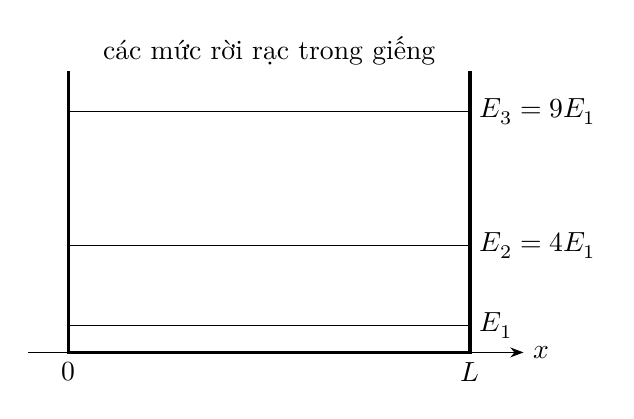
\begin{tikzpicture}[>=Stealth,scale=0.85]
\draw[->] (-0.6,0)--(6.8,0) node[right] {$x$};
\draw[very thick] (0,4.2)--(0,0)--(6,0)--(6,4.2);
\draw (0,0.4)--(6,0.4) node[right] {$E_1$};
\draw (0,1.6)--(6,1.6) node[right] {$E_2=4E_1$};
\draw (0,3.6)--(6,3.6) node[right] {$E_3=9E_1$};
\node[below] at (0,0) {$0$};\node[below] at (6,0) {$L$};
\node at (3,4.5) {các mức rời rạc trong giếng};
\end{tikzpicture}
\end{center}

\textbf{Bài 2-15:} hạt có khối lượng rất lớn so với electron nhưng vẫn dùng
mô hình giếng đề yêu cầu.
$E_1=h^2/(8mL^2)=mv_{\min}^2/2$ cho
$v_{\min}=h/(2mL)$.
Nếu biết vận tốc $v$, liên hệ
$mv=nh/(2L)$ cho $n\approx2mLv/h$; $n$ thực tế phải là số nguyên.
Với $n$ rất lớn, mức kế tiếp rất sát nhau tương đối: khó thấy tính lượng tử
ở thang chuyển động đó.

\subsection{Giếng thế: xác suất và photon chuyển mức}\label{sec:wellpractice}
\ex{bài 2-18: electron trong giếng rộng $10^{-10}\unit m$}
Muốn tìm ba mức thấp nhất, tính một mức gốc rồi nhân $n^2$:
\[
E_1\approx37{,}6\unit{eV},\qquad
E_2=4E_1\approx150{,}4\unit{eV},\qquad
E_3=9E_1\approx338{,}4\unit{eV}.
\]
Nếu electron phát photon khi $2\to1$:
\[
E_\gamma=E_2-E_1=3E_1\approx112{,}8\unit{eV},\qquad
\lambda=\frac{hc}{E_\gamma}\approx11{,}0\unit{nm}.
\]
\think{$\lambda\leftarrow$ chênh lệch mức
$\leftarrow E_n$ của \emph{giếng thế}, không phải công thức hydro.}

\textbf{Nếu hỏi xác suất trong một đoạn:}
\[
P(a,b)=\frac2L\int_a^b\sin^2\left(\frac{n\pi x}{L}\right)dx
=\frac{b-a}{L}
-\frac{\sin(2n\pi b/L)-\sin(2n\pi a/L)}{2n\pi}.
\]
Chẳng hạn $a=0,b=L/2$ thì các số hạng sin bằng 0, được $P=1/2$.
\textbf{Nút sóng} là nơi $\psi=0$; trong giếng có $n-1$ nút bên trong.
Đỉnh $|\psi|^2$ là nơi có mật độ xác suất cao, không phải điểm electron
buộc phải nằm ở đó.

\subsection{Hàng rào thế và xuyên hầm}\label{sec:tunnel}
\idea{Hàng rào là miền có thế năng cao hơn miền xung quanh.
Hạt cổ điển có $E<V_0$ không vượt qua; hàm sóng lượng tử có thể xuyên vào
rào hữu hạn, tạo xác suất truyền sang phía bên kia.}
Với rào chữ nhật cao $V_0$, rộng $a$, thế năng hai bên đều bằng 0,
$0<E<V_0$ và khối lượng không đổi:
\[
\kappa=\frac{\sqrt{2m(V_0-E)}}\hbar,\qquad
D=\left[1+\frac{V_0^2\sinh^2(\kappa a)}{4E(V_0-E)}\right]^{-1}.
\]
$D$ là hệ số truyền qua, tức tỉ số thông lượng xác suất truyền/tới;
$\kappa$ có đơn vị m$^{-1}$. Với rào đủ dày, $\kappa a\gg1$:
\[
D\approx\frac{16E(V_0-E)}{V_0^2}e^{-2\kappa a}.
\]
Nhiều bài ước lượng chỉ giữ thừa số mũ $D\sim e^{-2\kappa a}$.
Đây là gần đúng theo độ suy giảm, không phải công thức chính xác
cho mọi chiều dày. Phải xem đề yêu cầu ước lượng hay tính chính xác.

\begin{center}
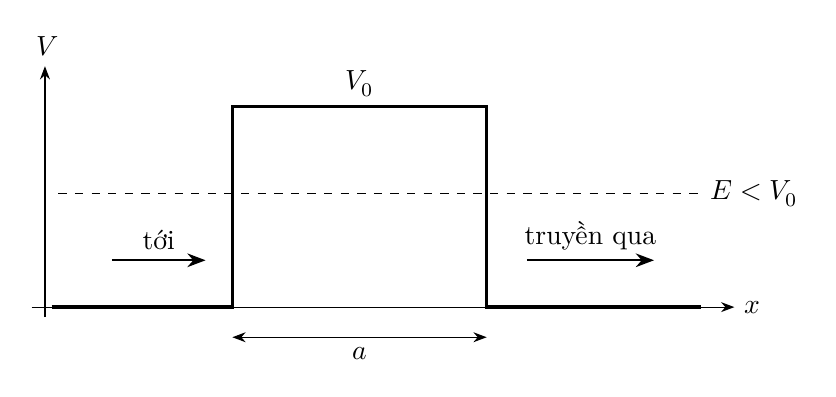
\begin{tikzpicture}[>=Stealth,scale=0.85]
\draw[->] (-2,0)--(8.5,0) node[right] {$x$};
\draw[->] (-1.8,-0.15)--(-1.8,3.6) node[above] {$V$};
\draw[very thick] (-1.7,0)--(1,0)--(1,3)--(4.8,3)--(4.8,0)--(8,0);
\draw[dashed] (-1.6,1.7)--(8,1.7) node[right] {$E<V_0$};
\node[above] at (2.9,3) {$V_0$};
\draw[<->] (1,-0.45)--(4.8,-0.45) node[midway,below] {$a$};
\draw[->,thick] (-0.8,0.7)--(0.6,0.7) node[midway,above] {tới};
\draw[->,thick] (5.4,0.7)--(7.3,0.7) node[midway,above] {truyền qua};
\end{tikzpicture}
\end{center}

\readit{Bài 2-16 cho $E=50\unit{eV}$, $V_0=70\unit{eV}$,
nên độ chênh trong căn là $20\unit{eV}$, không phải $70\unit{eV}$.
Đổi $20\unit{eV}$ sang J nếu dùng $m$ theo kg, $\hbar$ theo J\,s.}
\think{$D\leftarrow\kappa a\leftarrow m,V_0-E,a$.
Thay $a=1\unit{nm}$ và $0{,}1\unit{nm}$ riêng; chiều dày nằm trong số mũ
nên xác suất có thể khác nhau nhiều bậc độ lớn.}
\trap{Không dùng $h$ thay cho $\hbar$ trong $\kappa$.
Xuyên hầm không có nghĩa hạt mượn năng lượng để vượt rào;
năng lượng vẫn được bảo toàn trong mô hình thế tĩnh.}

\subsection{Dao động tử điều hòa và quay tử rắn}\label{sec:oscrotor}
\textbf{Dao động tử điều hòa} mô tả hạt trong thế parabol:
\[
V(x)=\frac12kx^2=\frac12m\omega^2x^2,\qquad
\omega=\sqrt{k/m},\qquad E_n=\hbar\omega(n+\tfrac12),\quad n=0,1,\ldots
\]
$k$ ở đây là độ cứng (N/m), không phải số sóng.
Các mức cách đều $\hbar\omega$.
Năng lượng điểm không $E_0=\hbar\omega/2$ là năng lượng thấp nhất,
không phải $mc^2$ dù cũng có thể được ký hiệu $E_0$ ở bài khác.
Hàm cơ bản đã chuẩn hóa:
\[
\psi_0(x)=\left(\frac{m\omega}{\pi\hbar}\right)^{1/4}
e^{-m\omega x^2/(2\hbar)}.
\]
Nếu đề hỏi kiểm tra nghiệm, đặt $\alpha=m\omega/\hbar$,
tính $\psi_0''=(\alpha^2x^2-\alpha)\psi_0$ rồi thế vào Schrödinger.
Hệ số đứng trước có thể sai chuẩn hóa mà hàm vẫn thỏa phương trình vi phân.

\textbf{Quay tử rắn} là hệ quay có khoảng cách giữa các phần không đổi.
Gọi $\mathcal I$ là mômen quán tính (kg\,m$^2$), $\mathcal I=\mu_rR^2$
với hai hạt cách nhau $R$ và khối lượng rút gọn
$\mu_r=m_1m_2/(m_1+m_2)$:
\[
E_\ell=\frac{\hbar^2}{2\mathcal I}\ell(\ell+1),\qquad \ell=0,1,2,\ldots
\]
\trap{Giếng thế bắt đầu $n=1$; dao động tử bắt đầu $n=0$;
quay tử có $\ell=0$. Phải nhận ra mô hình trước khi chọn số lượng tử thấp nhất.}

\subsection{Giá trị kỳ vọng và giao hoán: cách đọc câu lý thuyết}\label{sec:commute}
Giá trị kỳ vọng trong trạng thái đã chuẩn hóa:
\[
\langle A\rangle=\int\psi^*\hat A\psi\,dx,
\qquad \sigma_A=\sqrt{\langle A^2\rangle-\langle A\rangle^2}.
\]
Một phép đo không nhất thiết cho đúng giá trị kỳ vọng;
đó là trung bình qua nhiều phép đo trên các hệ cùng trạng thái.

\textbf{Giao hoán tử} đo sự khác nhau khi đổi thứ tự hai thao tác:
\[
[\hat A,\hat B]=\hat A\hat B-\hat B\hat A.
\]
Ví dụ $\hat x\hat p_x\psi=x(-i\hbar\psi')$,
còn $\hat p_x\hat x\psi=-i\hbar(x\psi)'=-i\hbar(\psi+x\psi')$.
Suy ra $[\hat x,\hat p_x]\psi=i\hbar\psi$.
Phải cho toán tử tác động lên một hàm thử để xử lý đúng quy tắc đạo hàm tích.

Các thành phần mômen động lượng thỏa
$[\hat L_x,\hat L_y]=i\hbar\hat L_z$ và các hoán vị vòng.
Với $\hat L_\pm=\hat L_x\pm i\hat L_y$:
$[\hat L_+,\hat L_-]=2\hbar\hat L_z$.
Các toán tử không giao hoán nói chung không có hệ trạng thái xác định
đồng thời mọi giá trị. Đây là mối nối giữa đại số toán tử và bất định.

\chap{Chương 3: nguyên tử, phổ và mômen từ}
\subsection{Mức năng lượng, trạng thái và phổ hydro}\label{sec:hydrogen}
\idea{Trạng thái là mô tả lượng tử của hệ; mức năng lượng là một giá trị
năng lượng cho phép. Nhiều trạng thái khác nhau có thể có cùng năng lượng,
gọi là suy biến. Phổ là tập các năng lượng hoặc các vạch chuyển mức.}
Với hydro trong mô hình cơ bản, bỏ qua các hiệu chỉnh tinh tế:
\[
E_n=-\frac{13{,}6}{n^2}\unit{eV},\qquad n=1,2,3,\ldots
\]
Mốc $E=0$ ứng với electron và proton tách xa vô hạn, không có động năng
tương đối. $E_n<0$ nghĩa là electron còn liên kết với nguyên tử.
$n$ càng lớn, $E_n$ càng gần 0 và năng lượng càng cao.

\textbf{Trạng thái cơ bản:} $n=1$, $E_1=-13{,}6\unit{eV}$.
\textbf{Kích thích:} đưa nguyên tử lên mức cao hơn nhưng chưa tách electron.
\textbf{Ion hóa:} tách electron khỏi trạng thái liên kết; năng lượng tối thiểu
từ mức $n$ là $E_{\rm ion}=0-E_n=13{,}6/n^2\unit{eV}$.

Nếu chuyển từ mức cao $n_i$ xuống mức thấp $n_f$:
\[
E_\gamma=E_{n_i}-E_{n_f}=hc/\lambda>0,
\qquad
\frac1\lambda=R_H\left(\frac1{n_f^2}-\frac1{n_i^2}\right).
\]
Phát xạ làm hệ mất năng lượng nhưng photon có năng lượng dương.
Hấp thụ là chiều chuyển ngược lại và cần năng lượng đúng độ chênh mức
trong mô hình lý tưởng.

\trap{Trong giếng vô hạn, $E_n$ tăng theo $n^2$; trong hydro, $E_n$ tăng
theo $-1/n^2$. Dấu âm không có nghĩa mức $n=1$ cao hơn mức $n=2$.}

\subsection{Dãy phổ, bước sóng ngắn nhất và dài nhất}\label{sec:series}
\textbf{Dãy phổ} gom các chuyển mức có cùng mức cuối khi phát xạ.
Lyman (Liman) có $n_f=1$; Balmer có $n_f=2$; Paschen có $n_f=3$.
\[
E_\gamma=hc/\lambda
\quad\Rightarrow\quad
\text{photon càng nhiều năng lượng, bước sóng càng ngắn.}
\]
Với $n_f$ cố định:
\begin{itemize}
\item $\lambda_{\max}$: chênh mức nhỏ nhất, $n_i=n_f+1$.
\item $\lambda_{\min}$: chênh mức lớn nhất trong dãy, giới hạn $n_i\to\infty$.
\end{itemize}

\ex{bài 3-1: dãy Lyman}
$n_f=1$. Vạch dài nhất là $2\to1$:
$1/\lambda_{\max}=R_H(1-1/4)=3R_H/4$.
Giới hạn ngắn nhất là $\infty\to1$:
$1/\lambda_{\min}=R_H$.
\[
\lambda_{\max}=\frac4{3R_H}\approx1216\unit{\mathring A},\qquad
\lambda_{\min}=\frac1{R_H}\approx912\unit{\mathring A}.
\]
\think{Muốn tìm cực trị bước sóng, tìm cực trị \emph{độ chênh năng lượng}
theo chiều ngược lại. Không cần đạo hàm.}

\ex{bài 3-2: suy năng lượng ion hóa từ giới hạn Balmer}
Giới hạn Balmer có $n_f=2,n_i\to\infty$ nên photon có năng lượng
$|E_2|=hc/\lambda_{\min}$. Vì $|E_1|=4|E_2|$,
\[
E_{\rm ion,1}=\frac{4hc}{\lambda_{\min}}.
\]
Với $3650\unit{\mathring A}=365\unit{nm}$, được khoảng $13{,}6\unit{eV}$.
Con số $hc/\lambda_{\min}$ riêng lẻ chỉ là ion hóa từ mức 2, chưa phải từ mức cơ bản.

\subsection{Kích thích bằng va chạm: tìm những vạch có thể phát}\label{sec:collision}
\idea{Electron tới có một lượng động năng. Nó chỉ có thể kích thích
nguyên tử lên mức mà độ tăng năng lượng không vượt lượng động năng đó.
Nguyên tử có thể trở về mức thấp qua nhiều bước, phát nhiều loại photon.}

\ex{bài 3-3: electron tới có động năng $12{,}2\unit{eV}$}
Giả sử nguyên tử hydro ban đầu ở mức cơ bản và bỏ qua động năng giật lùi
của toàn nguyên tử. Điều kiện để lên mức $n$:
\[
E_n-E_1=13{,}6\left(1-\frac1{n^2}\right)\unit{eV}
\le12{,}2\unit{eV}.
\]
Mức 3 cần khoảng $12{,}09\unit{eV}$; mức 4 cần $12{,}75\unit{eV}$,
nên mức cao nhất đạt được là $n=3$.

\begin{center}
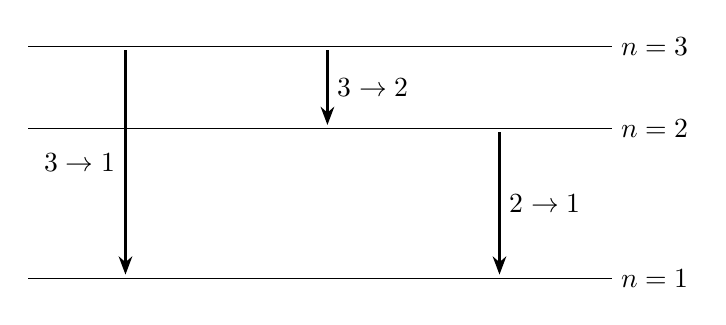
\begin{tikzpicture}[>=Stealth,scale=0.95]
\draw (0,0)--(7.8,0) node[right] {$n=1$};
\draw (0,2)--(7.8,2) node[right] {$n=2$};
\draw (0,3.1)--(7.8,3.1) node[right] {$n=3$};
\draw[->,thick] (1.3,3.05)--(1.3,0.05) node[midway,left] {$3\to1$};
\draw[->,thick] (4,3.05)--(4,2.05) node[midway,right] {$3\to2$};
\draw[->,thick] (6.3,1.95)--(6.3,0.05) node[midway,right] {$2\to1$};
\end{tikzpicture}
\end{center}

Liệt kê ba vạch trong mô hình bài tập:
$3\to1$ khoảng $102{,}6\unit{nm}$,
$3\to2$ khoảng $656\unit{nm}$,
$2\to1$ khoảng $121{,}6\unit{nm}$.
Số liệu cuối thay đổi nhẹ theo hằng số làm tròn.

\think{Các vạch $\leftarrow$ các cặp mức có thể chuyển xuống
$\leftarrow n_{\max}\leftarrow$ năng lượng electron tới và trạng thái đầu.}
\trap{Không đặt $E_\gamma=12{,}2\unit{eV}$ cho mọi vạch.
Electron tới có thể còn động năng sau va chạm. Với bài thực tế phân giải
trạng thái, còn phải xét quy tắc chọn; bài này dùng sơ đồ mức cơ bản của đề.}

\subsection{Bốn số lượng tử và orbital}\label{sec:qn}
\idea{Các số lượng tử là những nhãn phân loại trạng thái, đồng thời quyết
định các giá trị đo cho phép. Orbital là trạng thái không gian của electron,
không phải một quỹ đạo tròn mà electron phải chạy trên đó.}
\begin{tabularx}{\textwidth}{@{}Q{1.5cm}Q{3.5cm}Q{3.5cm}Y@{}}
\toprule
\textbf{Nhãn} & \textbf{Tên} & \textbf{Giá trị} & \textbf{Cho biết}\\\midrule
$n$ & Số lượng tử chính & $1,2,3,\ldots$ & Lớp; năng lượng hydro cơ bản.\\
$\ell$ & Số lượng tử quỹ đạo & $0,1,\ldots,n-1$ & Độ lớn mômen động lượng; phân lớp.\\
$m_\ell$ & Số lượng tử từ & $-\ell,\ldots,0,\ldots,+\ell$ & Hình chiếu mômen quỹ đạo.\\
$m_s$ & Số lượng tử từ spin & $-1/2,+1/2$ & Hình chiếu spin electron.\\
\bottomrule
\end{tabularx}

Electron luôn có số lượng tử spin $s=1/2$, nên thường chỉ cần ghi
bốn nhãn $n,\ell,m_\ell,m_s$.
Tên phân lớp: $\ell=0,1,2,3$ tương ứng $s,p,d,f$.
Chữ $s$ trong tên phân lớp không phải số lượng tử spin $s$.
Ví dụ $3p$ nghĩa là $n=3,\ell=1$; $m_\ell=-1,0,1$ tạo ba orbital không gian.

Với mỗi phân lớp có $2\ell+1$ orbital; mỗi orbital có thể chứa tối đa hai
electron spin đối nhau. Sức chứa phân lớp là $2(2\ell+1)$:
$s:2$, $p:6$, $d:10$, $f:14$. Cả lớp $n$ chứa tối đa $2n^2$ electron.

\checkit{Với $n=3$, $\ell$ có thể là 0, 1, 2; không thể là 3.
Với $\ell=2$, có năm giá trị $m_\ell$, nhưng vẫn chỉ một độ lớn mômen quỹ đạo.}

\subsection{Mômen động lượng: độ lớn khác hình chiếu}\label{sec:angular}
\idea{Trong cơ học cổ điển, mômen động lượng đo chuyển động quay:
$\vec L=\vec r\times\vec p$. Trong lượng tử, độ lớn và một hình chiếu có
các giá trị rời rạc xác định bởi $\ell,m_\ell$.}
\[
|\vec L|=\hbar\sqrt{\ell(\ell+1)},\qquad L_z=m_\ell\hbar.
\]
\textbf{Hình chiếu} $L_z$ là thành phần của vectơ theo trục $Oz$, có thể
hình dung như bóng của vectơ lên trục đó. Nó có dấu, nên không đồng nhất
với độ dài $|\vec L|$ luôn không âm.
Trong lời giải môn học, $\vec M_l$ thường chỉ chính $\vec L$.
Đơn vị mômen động lượng là J\,s, không phải đơn vị mômen lực N\,m.

\textbf{Bài 3-6: vẽ định hướng.} Với $\ell>0$, góc hình dung giữa
$\vec L$ và trục $Oz$ thỏa
\[
\cos\theta=\frac{L_z}{|\vec L|}
=\frac{m_\ell}{\sqrt{\ell(\ell+1)}}.
\]
Ví dụ $\ell=1$: độ dài vectơ biểu diễn là $\sqrt2\hbar$;
các hình chiếu là $-\hbar,0,+\hbar$, tương ứng các góc $135^\circ,90^\circ,45^\circ$.
Với $\ell=2$ có năm hình chiếu; với $\ell=3$ có bảy.
\textbf{Trường hợp $\ell=0$:} $\vec L=0$, không có hướng hoặc góc xác định;
không thay vào biểu thức $0/0$ để tìm góc.

Hình vectơ chỉ hỗ trợ hình dung lượng tử hóa hình chiếu. Không được diễn
giải nó như cả ba thành phần $L_x,L_y,L_z$ đều đồng thời có giá trị cổ điển xác định.

\think{Vẽ hướng $\leftarrow$ các $L_z$ và cùng một độ dài $|\vec L|$
$\leftarrow$ liệt kê $m_\ell$ ở $\ell$ đã cho.
Nếu chưa biết $\ell$, tìm nó từ điều kiện $0\le\ell\le n-1$.}

\subsection{Mômen từ quỹ đạo và magneton Bohr}\label{sec:moment}
\idea{Một điện tích chuyển động quay tạo hiệu ứng từ giống một vòng dòng
điện. Mômen từ cho biết cách hệ tương tác với từ trường ngoài.}
Với vòng dòng điện, $\mu=I_{\rm dòng}S$.
Electron chạy tròn bán kính $r$, tốc độ $v$ trong mô hình cổ điển:
\[
I_{\rm dòng}=\frac e{\tau}=\frac{ev}{2\pi r},\qquad
\mu=I_{\rm dòng}\pi r^2=\frac{evr}{2}.
\]
Lực Coulomb đóng vai trò hướng tâm:
$m_ev^2/r=e^2/(4\pi\varepsilon_0r^2)$.
\think{Bài 3-4 hỏi $\mu(r)$:
$\mu\leftarrow evr/2\leftarrow v(r)\leftarrow$ cân bằng hướng tâm với lực Coulomb.}

Trong lượng tử, với $e>0$:
\[
\vec\mu_L=-\frac{e}{2m_e}\vec L,\qquad
\mu_B=\frac{e\hbar}{2m_e},\qquad
|\vec\mu_L|=\mu_B\sqrt{\ell(\ell+1)},\quad
\mu_{Lz}=-m_\ell\mu_B.
\]
Dấu trừ nghĩa là mômen từ quỹ đạo electron ngược chiều mômen động lượng.
\textbf{Magneton Bohr} $\mu_B$ là đơn vị tự nhiên để biểu diễn mômen từ,
không phải tên một số lượng tử.

\ex{bài 3-5: các mômen từ có thể có khi $n=3$}
$n=3\Rightarrow\ell=0,1,2$, nên các \emph{độ lớn} là
\[
0,\qquad\sqrt2\mu_B,\qquad\sqrt6\mu_B.
\]
Nếu câu hỏi đổi thành \emph{hình chiếu}, phải liệt kê $-m_\ell\mu_B$
cho từng $\ell$, chứ không trả lời bằng ba độ lớn trên.

\subsection{Spin, tương tác từ và bài vạch 21 cm}\label{sec:spin}
\idea{Spin là mômen động lượng nội tại của electron. Đây không phải mô hình
một quả cầu nhỏ tự quay theo cơ học cổ điển. Electron có $s=1/2$ và hai
giá trị hình chiếu spin.}
\[
|\vec S|=\hbar\sqrt{s(s+1)}=\frac{\sqrt3}{2}\hbar,
\qquad S_z=m_s\hbar=\pm\frac\hbar2.
\]
Mômen từ spin xấp xỉ
$\vec\mu_s=-g_s(e/2m_e)\vec S$, $g_s\approx2$.
Trong mô hình của đề, lấy $g_s=2$ nên
$\mu_{sz}=\mp\mu_B$.

Năng lượng tương tác của mômen từ với từ trường:
\[
E_B=-\vec\mu\cdot\vec B.
\]
Nếu $\vec B$ theo trục $Oz$, hai hình chiếu spin có hai mức năng lượng
cách nhau $\Delta E=2\mu_BB$ trong mô hình electron spin $1/2$ này.

\readit{Bài 3-7 dùng photon $\lambda=21\unit{cm}=0{,}21\unit m$
do đổi trạng thái tương đối của spin electron và proton.
Bài yêu cầu một \emph{từ trường hiệu dụng} tác dụng lên electron trong
mô hình đã cho. Ta nối $hc/\lambda=2\mu_BB$:
\[
B=\frac{hc}{2\mu_B\lambda}\approx0{,}051\unit T.
\]
Không hiểu đây là phép đo trực tiếp một từ trường ngoài thực sự trong thiên hà.
Nguồn gốc vật lý đầy đủ của vạch là cấu trúc siêu tinh tế do tương tác
mômen từ electron và proton.}

\think{$B\leftarrow\Delta E/(2\mu_B)\leftarrow hc/\lambda$.
Hệ số 2 xuất hiện từ \emph{chênh lệch hai mức}, không phải năng lượng của một mức.}

\subsection{Nguyên tử nhiều electron, Pauli và cấu hình}\label{sec:configuration}
\textbf{Cấu hình electron} cho biết electron phân bố vào các phân lớp nào.
Ví dụ $1s^2\,2s^2\,2p^6$ có 10 electron; số mũ là số electron trong phân lớp.
Nguyên tử trung hòa có số electron bằng số hiệu nguyên tử $Z$.
Ion dương mất electron; ion âm nhận thêm electron.

\textbf{Nguyên lý Pauli:} không có hai electron trong một nguyên tử cùng
toàn bộ bốn số lượng tử $n,\ell,m_\ell,m_s$.
Do đó mỗi orbital chứa tối đa hai electron có spin đối nhau.
\textbf{Quy tắc Hund:} trong các orbital suy biến của một phân lớp,
electron chiếm riêng trước với spin song song rồi mới ghép đôi.
\textbf{Điền mức thấp trước:} thứ tự thực hành ở đây là
\[
1s,\ 2s,\ 2p,\ 3s,\ 3p,\ 4s,\ 3d,\ 4p,\ 5s,\ 4d,\ 5p.
\]
Đây là quy tắc gần đúng cho cấu hình cơ bản; một số nguyên tố có ngoại lệ.
Năm khí trơ đầu tiên của bài 3-9 không vướng các ngoại lệ điển hình đó.

\ex{bài 3-9: năm khí trơ đầu tiên}
\begin{tabularx}{\textwidth}{@{}Q{2.4cm}Q{1.2cm}Y@{}}
\toprule
\textbf{Nguyên tố} & $Z$ & \textbf{Cấu hình cơ bản}\\\midrule
He & 2 & $1s^2$\\
Ne & 10 & $1s^2\,2s^2\,2p^6$\\
Ar & 18 & $[\mathrm{Ne}]\,3s^2\,3p^6$\\
Kr & 36 & $[\mathrm{Ar}]\,3d^{10}\,4s^2\,4p^6$\\
Xe & 54 & $[\mathrm{Kr}]\,4d^{10}\,5s^2\,5p^6$\\
\bottomrule
\end{tabularx}
Ngoặc vuông thay cho toàn bộ cấu hình khí trơ trước đó.
Thứ tự \emph{ghi} có thể nhóm theo lớp khác thứ tự \emph{điền};
kiểm tra tổng số mũ bằng $Z$ và sức chứa từng phân lớp.

\subsection{Lớp đầy và ký hiệu trạng thái tổng hợp}\label{sec:term}
\idea{Khi xét cả nguyên tử, ta tổng hợp mômen của tất cả electron.
Các chữ hoa $L,S,J$ thường là số lượng tử tổng, không phải các vectơ
hay số lượng tử $\ell,s,j$ của riêng một electron.}
Trong ghép $LS$:
\[
\vec L_{\rm tổng}=\sum_i\vec L_i,\quad
\vec S_{\rm tổng}=\sum_i\vec S_i,\quad
\vec J_{\rm tổng}=\vec L_{\rm tổng}+\vec S_{\rm tổng}.
\]
Trong các tổng này, $\vec L_i,\vec S_i$ là các vectơ mômen của electron $i$;
các \emph{số lượng tử} tổng không cộng như các số vô hướng thông thường.
Ký hiệu số hạng phổ:
\[
{}^{2S+1}L_J.
\]
$2S+1$ là độ bội spin; chữ ở giữa mã hóa $L$:
$L=0,1,2,3$ ứng với $S,P,D,F$; chỉ số dưới là $J$.
Chữ $S$ ở giữa trong ${}^1S_0$ có nghĩa $L=0$, không phải spin bằng 1.

\textbf{Bài 3-8:} với phân lớp điền đầy, mọi $m_\ell$ đều được chiếm
đối xứng và mỗi orbital ghép đủ hai spin. Cấu trúc lớp kín cho tổng
mômen quỹ đạo $L=0$ và tổng spin $S=0$, do đó $J=0$.
\[
2S+1=1,\quad L=0\ \leftrightarrow\ S,\quad J=0
\quad\Rightarrow\quad{}^1S_0.
\]
\trap{Chỉ thấy tổng hình chiếu $M_L=0$ chưa đủ để kết luận $L=0$:
một trạng thái có $L>0$ vẫn có thể có hình chiếu 0.
Lập luận ở đây cần thêm điều kiện \emph{phân lớp điền đầy}, có tính đối xứng
và không còn mômen tổng chưa ghép.}

\subsection{Chuyển mức, cộng hưởng và laser: từ vựng lý thuyết}\label{sec:laser}
\textbf{Hấp thụ:} hệ nhận photon và đi lên mức cao, $h\nu=E_2-E_1$.
\textbf{Phát xạ tự phát:} hệ tự chuyển xuống, phát photon có pha và hướng
ngẫu nhiên giữa các sự kiện.
\textbf{Phát xạ kích thích / cưỡng bức:} photon tới kích thích hệ đang ở mức cao
phát thêm photon vào cùng mode bức xạ, cùng tần số, hướng, pha và phân cực
trong mô hình lý tưởng.

\textbf{Thời gian sống dài / trạng thái siêu bền} giúp tích lũy hạt ở mức cao.
\textbf{Nghịch đảo mật độ} nghĩa là mật độ mức trên lớn hơn mức dưới
khi hai mức có cùng độ suy biến; tổng quát là $N_2/g_2>N_1/g_1$,
với $g_i$ là số trạng thái suy biến của mức $i$.
\textbf{Bơm} là cung cấp năng lượng để tạo và duy trì phân bố đó.
\textbf{Hoạt chất} là môi trường tạo khuếch đại; \textbf{buồng cộng hưởng}
cho ánh sáng phản hồi nhiều lần. Laser cần độ khuếch đại thắng tổng tổn hao.

Với buồng hai gương cách $L$ và chiết suất gần như không đổi $n_r$,
điều kiện mode dọc là $2n_rL=q\lambda_0$, $q$ nguyên;
khoảng cách tần số mode gần $c/(2n_rL)$.
$\lambda_0$ là bước sóng trong chân không; đừng trộn với bước sóng trong môi trường.

\textbf{Cộng hưởng} xảy ra khi năng lượng photon khớp chênh lệch mức.
\textbf{Tách mức Zeeman} là tách năng lượng do từ trường.
Trong mô hình spin electron:
\[
h\nu=\Delta E\approx g_s\mu_BB.
\]
\textbf{Cộng hưởng cyclotron} liên quan chuyển động quỹ đạo trong từ trường,
$\omega_c=eB/m^*$; $m^*$ là khối lượng hiệu dụng của electron trong chất rắn.
\textbf{Mức Landau} là các mức lượng tử của chuyển động vuông góc $\vec B$,
cách nhau $\hbar\omega_c$ trong mô hình electron tự do hiệu dụng.
\textbf{Cộng hưởng từ hạt nhân} dùng các mức do mômen từ hạt nhân;
không thay trực tiếp khối lượng electron vào công thức cho hạt nhân.

\readit{Gặp câu lý thuyết về các hiện tượng này, trước hết xác định
\emph{hệ có những mức nào, tác nhân nào gây chuyển mức, năng lượng chuyển
mức lấy từ đâu}. Sau đó mới nhớ tên hiệu ứng hoặc công thức tần số.}

\chap{Tra theo bài tập và tự dựng lời giải}\label{sec:map}
\subsection{Chương 1: năm bài, ba mô hình}
\begin{tabularx}{\textwidth}{@{}Q{1.4cm}Q{3.4cm}YQ{1.5cm}@{}}
\toprule
\textbf{Bài} & \textbf{Mục tiêu} & \textbf{Chuỗi cần dựng} & \textbf{Đọc mục}\\\midrule
1-1 & Độ nhạy tĩnh điện & $S_E\leftarrow D/U_k\leftarrow$ gia tốc ngang và thời gian bay. & \ref{sec:crt}\\
1-2 & Độ nhạy theo dòng cuộn & $S_I\leftarrow D/I\leftarrow r,B/I,v\leftarrow$ cuộn và thế tăng tốc. & \ref{sec:magnetic}\\
1-3 & Hội tụ và tiêu cự lưới cầu & $f\leftarrow y/\delta\leftarrow$ góc khúc xạ và pháp tuyến. & \ref{sec:lens}\\
1-4 & Điện thế diapham & $U_D\leftarrow f=d_2\leftarrow$ độ dốc điện thế hai phía. & \ref{sec:diaphragm}\\
1-5 & Điện thế diapham thứ hai & $U_2\leftarrow$ ảnh ở anot $\leftarrow f_1,f_2$ và khoảng cách. & \ref{sec:diaphragm}\\
\bottomrule
\end{tabularx}

\subsection{Chương 2: mười tám bài}
\begin{tabularx}{\textwidth}{@{}Q{1.3cm}Q{3.2cm}YQ{1.6cm}@{}}
\toprule
\textbf{Bài} & \textbf{Mục tiêu} & \textbf{Chuỗi cần dựng} & \textbf{Đọc mục}\\\midrule
2-1 & Thời gian tích lũy & $t\leftarrow\varphi/P_a\leftarrow I_{\rm bx},S_a$. & \ref{sec:photon}\\
2-2 & Động năng, số electron & $K_{\max}\leftarrow E_\gamma-\varphi$; $\Phi_e\leftarrow I_{\rm bx}/E_\gamma$. & \ref{sec:photoelectric}\\
2-3 & Vận tốc giật lùi & $v_e\leftarrow K_e\leftarrow E_\gamma'$; bảo toàn cả năng lượng và động lượng. & \ref{sec:compton}\\
2-4 & Thế tăng tốc & $U\leftarrow K/e\leftarrow p=h/\lambda$. & \ref{sec:debroglie}\\
2-5 & Giới hạn năng lượng lớn & $\lambda\leftarrow h/p$ và $pc\approx\mathcal E$. & \ref{sec:debroglie}\\
2-6 & Vận tốc pha, nhóm & $v_{\rm pha}\leftarrow E/p$; $v_{\rm nhóm}\leftarrow dE/dp$; nêu quy ước $E$. & \ref{sec:phase}\\
2-7 & Bán kính vòng nhiễu xạ & $r\leftarrow2\theta\leftarrow\lambda\leftarrow K$. & \ref{sec:diffraction}\\
2-8 & Khoảng vân & $i\leftarrow\lambda L/d\leftarrow h/(mv)$; giữ $h$ giả định. & \ref{sec:diffraction}\\
2-9 & Bất định vị trí & $\Delta x\leftarrow C/\Delta p\leftarrow10^{-3}p$. & \ref{sec:uncertainty}\\
\bottomrule
\end{tabularx}

\begin{tabularx}{\textwidth}{@{}Q{1.3cm}Q{3.2cm}YQ{1.6cm}@{}}
\toprule
\textbf{Bài} & \textbf{Mục tiêu} & \textbf{Chuỗi cần dựng} & \textbf{Đọc mục}\\\midrule
2-10 & Thời gian sống & $\tau\leftarrow\Delta E\leftarrow\lambda,\Delta\lambda$; xác định quy ước độ rộng. & \ref{sec:lifetime}\\
2-11 & Liên hệ với bước sóng & $\Delta x\leftarrow C/\Delta p$ với $\Delta p=p=h/\lambda$. & \ref{sec:uncertainty}\\
2-12 & Liên hệ năng lượng-thời gian & $\Delta K\approx v\Delta p$; $\Delta t=\Delta x/v$. & \ref{sec:lifetime}\\
2-13 & Năng lượng giam giữ & $K\leftarrow p\sim\hbar/L$; kiểm tra tương đối tính. & \ref{sec:confinement}\\
2-14 & Hàm riêng, phổ động lượng & Giải $\hat A\psi=a\psi$; xem miền và điều kiện biên. & \ref{sec:operator}\\
2-15 & Vận tốc nhỏ nhất, $n$ & $v_{\min}\leftarrow E_1$; $n\leftarrow mv=nh/(2L)$. & \ref{sec:well}\\
2-16 & Xác suất xuyên hầm & $D\leftarrow\kappa a\leftarrow V_0-E,m,a$. & \ref{sec:tunnel}\\
2-17 & Biên độ chuẩn hóa & $A\leftarrow\int_0^L|\psi|^2dx=1$. & \ref{sec:wavefunction}\\
2-18 & Mức năng lượng, photon & $E_n\leftarrow n^2E_1$; $\lambda\leftarrow hc/(E_2-E_1)$. & \ref{sec:wellpractice}\\
\bottomrule
\end{tabularx}

\subsection{Chương 3: chín bài}
\begin{tabularx}{\textwidth}{@{}Q{1.3cm}Q{3.2cm}YQ{1.6cm}@{}}
\toprule
\textbf{Bài} & \textbf{Mục tiêu} & \textbf{Chuỗi cần dựng} & \textbf{Đọc mục}\\\midrule
3-1 & Hai giới hạn Lyman & Cố định $n_f=1$; xét $n_i=2$ và $n_i\to\infty$. & \ref{sec:series}\\
3-2 & Năng lượng ion hóa & $|E_1|\leftarrow4|E_2|\leftarrow4hc/\lambda_{\min}$. & \ref{sec:series}\\
3-3 & Các vạch phát ra & Vạch $\leftarrow$ cặp mức $\leftarrow n_{\max}\leftarrow K_{\rm tới}$. & \ref{sec:collision}\\
3-4 & Mômen từ cổ điển & $\mu\leftarrow IS\leftarrow v(r)\leftarrow$ lực Coulomb và hướng tâm. & \ref{sec:moment}\\
3-5 & Các độ lớn mômen từ & $\mu_L\leftarrow\ell(\ell+1)\leftarrow\ell=0,1,2$ khi $n=3$. & \ref{sec:moment}\\
3-6 & Hình định hướng & $\theta\leftarrow L_z/|L|\leftarrow m_\ell,\ell$. & \ref{sec:angular}\\
3-7 & Từ trường hiệu dụng & $B\leftarrow\Delta E/(2\mu_B)\leftarrow hc/\lambda$. & \ref{sec:spin}\\
3-8 & Chứng minh ${}^1S_0$ & Lớp đầy $\Rightarrow L=S=0\Rightarrow J=0$. & \ref{sec:term}\\
3-9 & Cấu hình năm khí trơ & Số electron $Z$; điền phân lớp theo thứ tự và sức chứa. & \ref{sec:configuration}\\
\bottomrule
\end{tabularx}

\subsection{Khi chưa biết bắt đầu: chọn câu hỏi nhỏ hơn}
\begin{enumerate}
\item \textbf{Không hiểu câu chữ:} khoanh cụm từ, hỏi nó là vật, quá trình,
đại lượng hay điều kiện. Ví dụ \emph{công thoát} là năng lượng, không phải lực.
\item \textbf{Biết từ nhưng chưa biết ký hiệu:} viết tên đại lượng và đơn vị
trước; ký hiệu có thể tự đặt miễn nhất quán.
\item \textbf{Biết mục tiêu nhưng thiếu công thức:} hỏi đại lượng đó được
định nghĩa thế nào. Độ nhạy là tỉ số; xác suất là tích phân mật độ;
bước sóng photon nối với năng lượng.
\item \textbf{Có nhiều công thức:} chọn theo mô hình và điều kiện áp dụng.
Đặc biệt kiểm tra photon/hạt, cổ điển/tương đối tính, giếng/hydro/dao động tử.
\item \textbf{Đã có công thức nhưng còn thiếu biến:} coi biến thiếu là
mục tiêu trung gian rồi tiếp tục suy ngược, đến khi chạm dữ kiện đề cho.
\end{enumerate}

\subsection{Mẫu tự giải thích sau mỗi bài}
\textbf{Viết ba câu bằng lời của bạn:}
\begin{enumerate}
\item Bài này mô tả hiện tượng gì và dùng mô hình nào?
\item Đại lượng cần tìm nối với dữ kiện qua những bước nào?
\item Điều kiện nào làm cho các công thức mình dùng hợp lệ?
\end{enumerate}
Nếu chưa nói được một trong ba câu, đó là chỗ nên hỏi trợ giảng.
Khi hỏi, ghi số bài, dòng đang vướng và điều bạn đang nghĩ.
Không cần đợi đến khi biết giải một nửa bài mới hỏi.

\chap{Những điểm cần đối chiếu và nguồn tham khảo}
\subsection{Các khác biệt đã nhận diện trong bộ tài liệu}
\begin{itemize}
\item \textbf{Số bài Chương 2:} bài toán toán tử $i\,d/dx$ là 2-14 trong đề,
nhưng phần tương ứng có thể xuất hiện dưới nhãn 2-16 trong lời giải.
Xuyên hầm là 2-16 trong đề nhưng có nơi mang nhãn 2-17;
chuẩn hóa giếng cũng có thể cùng mang nhãn 2-17. Đối chiếu nội dung.
\item \textbf{Bài 2-10:} bản đề biên soạn dùng $4000\unit{\mathring A}$ và
$10^{-4}\unit{\mathring A}$; bản lời giải biên soạn dùng bộ số khác.
Không lấy kết quả của lời giải làm bằng chứng dữ kiện đề đúng hay sai.
\item \textbf{Bất định:} slide Chương II ghi $h/(4\pi)$;
một số lời giải cũ dùng $h/(2\pi)$. Xem mục \ref{sec:uncertainty},
phân biệt quan hệ chuẩn với ước lượng và quy ước bài học.
\item \textbf{Bài 2-13:} đề hỏi electron trong hạt nhân; một lời giải
biên soạn lại nói nucleon. Không đổi loại hạt khi tính.
Electron ở kích thước này cần kiểm tra tương đối tính.
\item \textbf{Bài 3-6:} đề biên soạn hỏi $\ell=0,1,2,3$;
lời giải có thể vẽ thêm $\ell=4$. Trường hợp $\ell=0$ có mômen bằng 0,
không có góc định hướng xác định.
\item \textbf{Độ dốc điện thế và điện trường:} một số lời giải dùng chữ
$E_i$ cho $(U_{i+1}-U_i)/d$. Sổ tay đổi thành $g_i$ để tách khỏi
điện trường vật lý $E_z=-d\Phi/dz$; xem mục \ref{sec:diaphragm}.
\end{itemize}
Tài liệu có sẵn đủ để học, nhưng mỗi công thức vẫn cần kiểm tra về ký hiệu,
đơn vị và giả thiết. Các điểm trên nhằm giúp bạn đọc nhất quán, không phải
một bản kiểm định toàn bộ mọi lời giải trong thư mục.

\subsection{Tài liệu nền trong thư mục VLDT/}
\begin{enumerate}
\item \texttt{docs/slides/latex/baitap.tex}: nội dung và số thứ tự bài tập
Chương 1--3; là bản chỉ mục bài dùng trong sổ tay.
\item \texttt{docs/slides/latex/giai-bt.tex} và
\texttt{docs/slides/tailieu-goc/giai-bt-goc.pdf}: đối chiếu lời giải,
đồng thời kiểm tra các chỗ lệch số bài và quy ước.
\item \texttt{docs/slides/Chương II\_ Cơ học lượng tử.pdf}:
slide nền của photon, sóng de Broglie, bất định, toán tử và các mô hình lượng tử.
\item \texttt{docs/slides/tailieu-goc/theory.pdf}:
khung ôn lý thuyết, quang học điện tử, chuyển mức, cộng hưởng và laser.
\item \texttt{docs/slides/latex/CT.tex} và
\texttt{src/midterm/latex/midterm.tex}: tham khảo dạng câu hỏi, thuật ngữ
và các công thức đang dùng; không mặc nhiên chép mọi biểu thức.
\end{enumerate}

\subsection{Nguồn đối chiếu thêm}
Các giải thích và ví dụ tính trong sổ tay được diễn giải lại cho mục tiêu
học của bạn. Ba nguồn sau hỗ trợ kiểm tra các điểm kỹ thuật cụ thể:
\begin{enumerate}
\item \href{https://www.mit.edu/~ashrstnv/uncertainty-principle.html}{MIT-hosted notes: Uncertainty principle}.
Đối chiếu định nghĩa bất định bằng độ lệch chuẩn và cận $\hbar/2$
ở mục \ref{sec:uncertainty}.
\item \href{https://ocw.mit.edu/courses/2-57-nano-to-macro-transport-processes-spring-2012/2e4ecaa5cf55f03bcefbc8ccce79aed6_MIT2_57S12_lec_notes_2004.pdf}{MIT OpenCourseWare: Nano-to-Macro Transport Processes, Lecture 13, tr. 95}.
Đối chiếu hệ số truyền qua rào chữ nhật và giới hạn rào dày
ở mục \ref{sec:tunnel}.
\item \href{https://physics.nist.gov/Pubs/AtSpec/node03.html}{NIST: Atomic States, Shells, and Configurations}.
Đối chiếu nhãn trạng thái một electron, phân lớp và tính chất tổng
mômen của phân lớp kín ở mục \ref{sec:qn} và \ref{sec:term}.
\end{enumerate}
\end{document}
